% !TEX root = handbook-physics.tex
%!TEX TS-program = pdflatex
%!TEX encoding = UTF-8 Unicode

\chapter{Kinetic Theory of Gases}
\label{ch-10}
\zhtitle{气体动理论}


\section{Certain Information on Classical Statistical Physics}
\label{sec-10.1}
\zhtitle{关于经典统计物理学的若干知识}

\subsection{}\label{10.1.1}The \redem{kinetic theory of gases} deals with the structure and physical properties of gases and is based on the statistical method of investigation \ssect{8.2.2}. Besides those mentioned in \ssect{8.2.1}, the following propositions form the foundation for \redem{classical statistical physics}.
\zhpar{\redem{气体动理论}研究气体的结构和物理性质，它以统计方法 \ssect{8.2.2} 为研究手段。除 \ssect{8.2.1} 中提到的各项内容外，下列命题构成了\redem{经典统计物理学}的基础。}

\subsection{}\label{10.1.2} A system of particles complies with the laws of conser­vation of energy \ssect{9.2.7}, momentum \ssect{2.7.1} and of angular momentum \ssect{4.4.1}. A system of charged particles complies with the law of conservation of electric charge \ssect{14.1.3}. 
\zhpar{质点系遵从能量守恒定律 \ssect{9.2.7}、动量守恒定律 \ssect{2.7.1} 和角动量守恒定律 \ssect{4.4.1}。带电质点系还遵从电荷守恒定律 \ssect{14.1.3}。}

\subsection{}\label{10.1.3} All physical processes in a system of particles proceed \redem{continuously} in space and time. A space-time description of any physical phenomena in classical mechanics and classical sta­tistical physics assumes the possibility of continuous variation of all physical quantities that characterize the state of the system. For instance, the velocity and energy of any particle can vary continuously due to the action of various forces. 
\zhpar{质点系中的所有物理过程都在空间和时间中\redem{连续}进行。经典力学和经典统计物理学对任何物理现象的时空描述，都假定表征系统状态的所有物理量均可连续变化。例如，任一质点的速度和能量都可以因各种力的作用而连续变化。}

\subsection{}\label{10.1.4} Each particle in a system is regarded as being ``tagged]]. It can be distinguished from all other such particles (\redem{distinguishability of identical particles in classical statistical physics}). 
\zhpar{质点系中的每个质点都被看作是“有标记的”，因而可以与系统中所有其他质点相区分（\redem{经典统计物理学中全同粒子的可区分性}）。}

\subsection{}\label{10.1.5} Any particle of a system can have arbitrary values for its coordinates and momenta (or velocities) independently of the values of these quantities for other particles of the system. If an infinitely small volume $\dd x \,\dd y \, \dd z$ is chosen in the coor­dinate system $XYZ$, any particle can be located within this volume regardless of the presence in this volume of any arbi­trary number of other particles. Likewise, any particle may be located within an arbitrary element of ``volume'' $\dd p_{x}\, \dd p_{y}\, \dd p_{z}$ of momentum space (or $\dd u_{x}\, \dd u_{y}\, \dd u_{z}$ of velocity space) regardless of the presence in these ``volumes'' of any arbitrary number of other particles. This implies that any particle can have momen­tum components along the coordinate axes within the limits from $p_{x}$ to $p_{x} + \dd p_{x}$, from $p_{y}$ to $p_{y} + \dd p_{y}$ and from $p_{z}$ to $p_{z} + \dd p_{z}$ (and, respectively, velocity components of the par­ticle along the coordinate axes within the limits from $u_{x}$ to $u_{x} + \dd u_{x}$, $u_{y}$ to $u_{y} + \dd u_{y}$, $u_{z}$ to $u_{z} + \dd u_{z}$). The minimum values of the volumes $\dd x \,\dd y \, \dd z$ and $\dd p_{x}\, \dd p_{y}\, \dd p_{z}$ are not restricted in any manner.
\zhpar{系统中任一质点的坐标和动量（或速度）都可以任意取值，而与系统中其他质点的这些量的取值无关。在坐标系 $XYZ$ 中取一无穷小体积元 $\dd x \,\dd y \, \dd z$，无论该体积元内有任意多个其他质点，任一质点都可以位于其中。同样，无论动量空间（或速度空间）的某一体积元 $\dd p_{x}\, \dd p_{y}\, \dd p_{z}$（或 $\dd u_{x}\, \dd u_{y}\, \dd u_{z}$）内有任意多个其他质点，任一质点都可以处于其中。这意味着，任一质点沿各坐标轴的动量分量可分别在 $p_{x}$ 到 $p_{x} + \dd p_{x}$、$p_{y}$ 到 $p_{y} + \dd p_{y}$ 以及 $p_{z}$ 到 $p_{z} + \dd p_{z}$ 的范围内取值（相应地，其沿各坐标轴的速度分量可分别在 $u_{x}$ 到 $u_{x} + \dd u_{x}$、$u_{y}$ 到 $u_{y} + \dd u_{y}$、$u_{z}$ 到 $u_{z} + \dd u_{z}$ 的范围内取值）。体积元 $\dd x \,\dd y \, \dd z$ 和 $\dd p_{x}\, \dd p_{y}\, \dd p_{z}$ 的最小值不受任何限制。}

\ssect{10.1.2} and \ssect{10.1.3} apply not only to classical statistical physics, they are characteristic of all of classical physics. Sections \ssect{10.1.4} and \ssect{10.1.5} apply only to classical statistical physics; they do not hold for quantum statistics \ssect{41.1.1}.
\zhpar{\ssect{10.1.2} 和 \ssect{10.1.3} 不仅适用于经典统计物理学，而且是整个经典物理学的共同特征。\ssect{10.1.4} 和 \ssect{10.1.5} 只适用于经典统计物理学，它们在量子统计中不成立 \ssect{41.1.1}。}

\section[Basic Equation]{Basic Equation of the Kinetic Theory of Gases}
\label{sec-10.2}
\zhtitle{气体动理论的基本方程}


\subsection{}\label{10.2.1} The pressure of a gas \ssect{8.3.2} in a vessel is the result of the collisions of the gas molecules with the walls of the vessel. The pressure of a gas is the macroscopic effect of the thermal motion of molecules \ssect{8.1.1}. As the molecules of the gas strike the walls of the vessel \ssect{8.4.1} they impart their momentum \ssect{2.3.4} to the walls. This change in momentum of the molecules exerts the pressure on the walls. For an ideal gas the collisions between the molecules within the vessel has no effect on the pressure exerted by the gas on the walls. Owing to the chaotic nature of thermal motion of the molecules \ssect{8.1.3} the pressure of the gas is the same on all the walls and, by definition \ssect{8.3.2}, is the average force exerted normal to unit area of the wall surface.
\zhpar{气体在容器中的压强是气体分子与器壁碰撞的结果。气体压强是分子热运动的宏观表现 \ssect{8.1.1}。气体分子撞击器壁 \ssect{8.4.1} 时，将其动量 \ssect{2.3.4} 传递给器壁，分子动量的这种变化对器壁产生压强。对于理想气体，分子之间的碰撞对气体作用于器壁的压强没有影响。由于分子热运动的无规则性 \ssect{8.1.3}，气体对各器壁的压强处处相同，并且按定义 \ssect{8.3.2}，压强即为垂直作用于单位器壁面积上的平均力。}

\subsection{}\label{10.2.2} The \redem{basic equation of the kinetic theory of gases} is 
\zhpar{气体动理论的\redem{基本方程}为}
\begin{equation*}%
pV = \frac{2}{3} E_{k},
\end{equation*}
where $p$ is the pressure of the gas, $V$ is its volume and $E_{k} = \sum_{i=1}^{N}
\frac{m_{i}u_{i}^{2}}{2}$ is total kinetic energy of translational motion of all the $N$ molecules of gas in the vessel.
\zhpar{式中 $p$ 为气体的压强，$V$ 为其体积，$E_{k}$ 为容器中全部 $N$ 个气体分子平动动能的总和。}

\subsection{}\label{10.2.3} In a homogeneous gas $m_{i} = m$, i.e. the mass of each molecule is the same, hut their velocities $u_{i}$ differ \ssect{10.3.1}, and
\zhpar{在均匀气体中，$m_{i} = m$，即各分子的质量相同，但它们的速度 $u_{i}$ 互不相同 \ssect{10.3.1}，并且}
\begin{equation*}%
E_{k} = \frac{m}{2} \sum_{i=1}^{N} u_{i}^{2},
\end{equation*}
It proves expedient to introduce the root-mean-square velocity $v_{\textrm{rms}}$ of translational motion of gases:
\zhpar{为便于讨论，引入气体平动的方均根速率 $v_{\textrm{rms}}$：}
\begin{equation*}%
v_{\textrm{rms}} = \sqrt{\frac{1}{N}\sum_{i=1}^{N}u_{i}^{2}},
\end{equation*}
where $N$ is the total number of molecules in volume $V$ of the gas. The root-mean-square velocity pertains to the whole population of molecules, but is meaningless in application to a single molecule or to a small number of molecules. Making use of $v_{\textrm{rms}}$ the expression for $E_{k}$ assumes the form
\zhpar{式中 $N$ 为气体在体积 $V$ 内的分子总数。方均根速率针对全体分子而言，对单个分子或少量分子则没有意义。利用 $v_{\textrm{rms}}$，$E_{k}$ 的表达式可写成下列形式：}
\begin{equation*}%
E_{k} = \frac{1}{2}Nm v_{\textrm{rms}}^{2} \qand pV = \frac{1}{3}Nm v_{\textrm{rms}}^{2} = \frac{1}{3}M v_{\textrm{rms}}^{2},
\end{equation*}
where $M = Nm$ is the mass of the gas.
\zhpar{式中 $M = Nm$ 为气体的质量。}

The basic equation for the pressure of a gas is
\zhpar{气体压强的基本方程为}
\begin{equation*}%
p = \frac{2}{3} E_{k_{0}} = \frac{1}{3} n_{0}mv_{\textrm{rms}}^{2} = \frac{1}{3} \rho v_{\textrm{rms}}^{2},
\end{equation*}
where $E_{k_{0}}= E_{k}/V$, $n_{0}= N/V$ is the number of molecules in unit volume, and $\rho = n_{0}m$ is the density of the gas.
\zhpar{式中 $E_{k_{0}}= E_{k}/V$，$n_{0}= N/V$ 为单位体积内的分子数，$\rho = n_{0}m$ 为气体的密度。}


\subsection{}\label{10.2.4} From a comparison of the Mendeleev-Clapeyron equation \ssect{8.4.4} with the basic equation \ssect{10.2.3} $RT = \mu v_{\textrm{rms}}^{2}/3$ it follows that
\zhpar{将门捷列夫-克拉珀龙方程 \ssect{8.4.4} 与基本方程 \ssect{10.2.3} 中的 $RT = \mu v_{\textrm{rms}}^{2}/3$ 相比较可知}
\begin{equation*}%
v_{\textrm{rms}} = \sqrt{\frac{3RT}{\mu}} = \sqrt{\frac{3RT}{m N_{A}}} = \sqrt{\frac{3kT}{m}} = 1.73 \sqrt{pv},
\end{equation*}
where $k$ is Boltzmann's constant \ssect{8.4.5}, $m$ is the mass of a mol­ecule, $N_{A}$ is Avogadro's number (Appendix~II), $p$ is the pres­sure of the gas, and $v$ is its specific volume.
\zhpar{式中 $k$ 为玻尔兹曼常量 \ssect{8.4.5}，$m$ 为分子的质量，$N_{A}$ 为阿伏伽德罗常量（见附录 II），$p$ 为气体的压强，$v$ 为其比容。}
\begin{marginfigure}%[!ht]
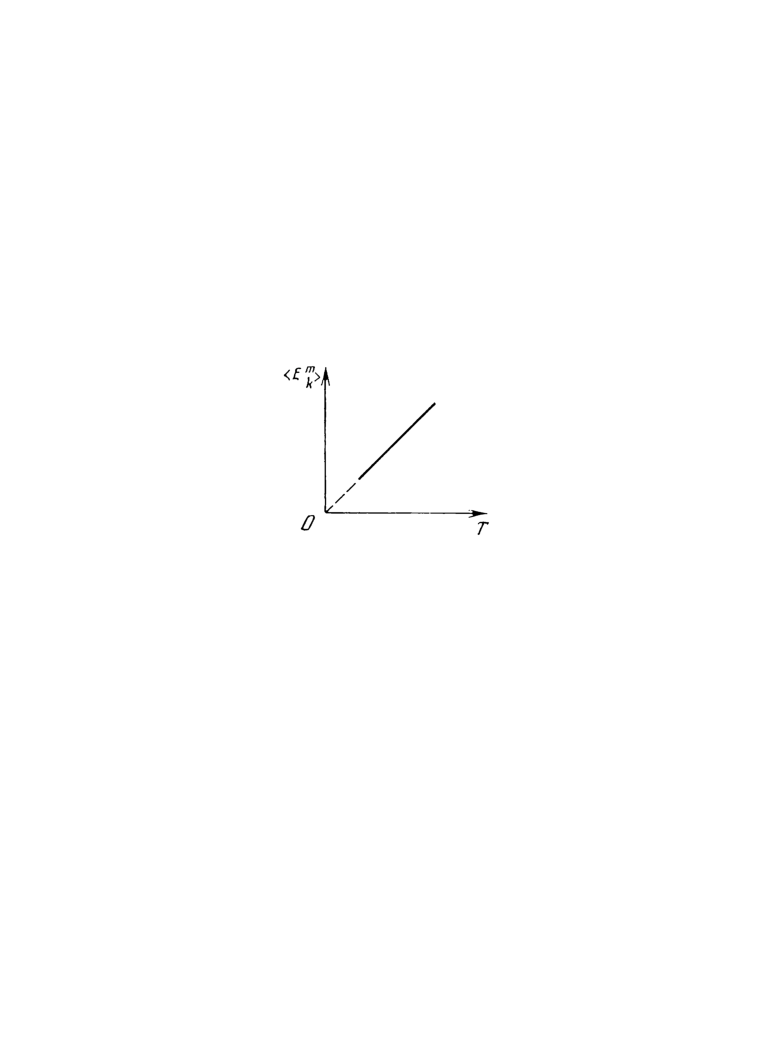
\includegraphics[width=0.8\textwidth]{figs/ch-10/fig-10-01.pdf}
\sidecaption{The relation of average kinetic energy and absolute temperature. \zhcap{平均动能与热力学温度的关系。}\label{fig-10-01}}
\end{marginfigure}

\subsection{}\label{10.2.5} The \redem{average kinetic energy of translational motion of the molecules in an ideal gas} is
\zhpar{理想气体中分子平动的\redem{平均动能}为}
\begin{equation*}%
v_{\textrm{rms}} = \sqrt{\frac{3RT}{\mu}} = \sqrt{\frac{3RT}{m N_{A}}} = \sqrt{\frac{3kT}{m}} = 1.73 \sqrt{pv}.
\end{equation*}
The average kinetic energy $\expval{E_{k}^{m}}$ is proportional to the abso­lute temperature and is independent of any other variables (\figr{fig-10-01}). 
The absolute, or thermodynamic, temperature is a measure of the average kinetic energy of translational motion of the molecules in an ideal gas. This consequence of the kinetic theory of gases is not valid in the region of ultra-low tempera­tures, close to absolute zero \ssect{8.3.4}.
\zhpar{平均动能 $\expval{E_{k}^{m}}$ 与绝对温度成正比，且与其他任何变量无关（见 \figr{fig-10-01}）。热力学温度（即绝对温度）是理想气体中分子平动平均动能的量度。气体动理论的这一结论在接近绝对零度的极低温区域内不成立 \ssect{8.3.4}。}

\section[Maxwell's Distribution Law]{Maxwell's Molecular Velocity and Energy Distribution Law (Maxwell's Distribution Law)}
\label{sec-10.3}
\zhtitle{麦克斯韦分子速度和能量分布律（麦克斯韦分布律）}


\subsection{}\label{10.3.1} The \redem{law of the distribution of molecular velocities for an ideal gas}, theoretically established by Maxwell, determines the number $\dd n$ of molecules of a homogeneous monatomic ideal gas, out of the total number $n_{0}$ of its molecules in unit volume, that has a velocity, at a given temperature, lying within the range from $u$ to $u + \dd u$. This law is valid for gases in a state of thermodynamic equilibrium \ssect{8.3.3}. The velocity distribution of the molecules of such a gas is a steady-state value. The Maxwellian distribution is based on pairwise collisions of the randomly moving gas molecules. This assumes uniform distribution of the molecules throughout the volume of the vessel, i.e. constant density of the gas.
\zhpar{由麦克斯韦从理论上建立的理想气体分子速度分布律，给出了在给定温度下，单位体积内总分子数 $n_{0}$ 中，速率位于 $u$ 到 $u + \dd u$ 范围内的分子数 $\dd n$（适用于均匀单原子理想气体）。该定律适用于处于热力学平衡态 \ssect{8.3.3} 的气体，这类气体的分子速度分布是稳定的。麦克斯韦分布以气体分子无规则运动中的两两碰撞为基础，并假定分子在容器整个体积内均匀分布，即气体密度处处一致。}

\subsection{}\label{10.3.2} In its most customary form, the law of the distribution of molecular speeds (magnitudes of the molecular velocities) is presented as
\zhpar{分子速率（即分子速度的大小）分布律最常用的形式为}
\begin{equation*}%
\dd n =n_{0} \left(\frac{m}{2 \pi k T}\right)^{3/2} \exp \left( - \frac{mu^{2}}{2kT}\right) 4 \pi u^{2} \dd u.
\end{equation*}
Here $u$ is the magnitude of the molecular velocity (speed of a molecule), $m$ is the mass of a molecule, $k$ is Boltzmann's constant, and $T$ is the absolute (thermodynamic) temperature. Molecular velocity distribution curves for various temperatures $T_{1}< T_{2} < T_{3}$ are shown in \figr{fig-10-2}. As is evident from these curves, the most probable velocity $u_{\textrm{p}}$ \ssect{10.3.4} increases with temperature and the fraction of molecules travelling at this velocity decreases.
\zhpar{式中 $u$ 为分子速度的大小（即分子速率），$m$ 为分子质量，$k$ 为玻尔兹曼常量，$T$ 为热力学（绝对）温度。不同温度 $T_{1}< T_{2} < T_{3}$ 下的分子速率分布曲线如 \figr{fig-10-2} 所示。由图中曲线可以看出，最概然速率 $u_{\textrm{p}}$ \ssect{10.3.4} 随温度升高而增大，而以该速率运动的分子所占的比例则减小。}
\begin{figure}%[!ht]
%\begin{wrapfigure}{r}{0.5\linewidth}
%\centering
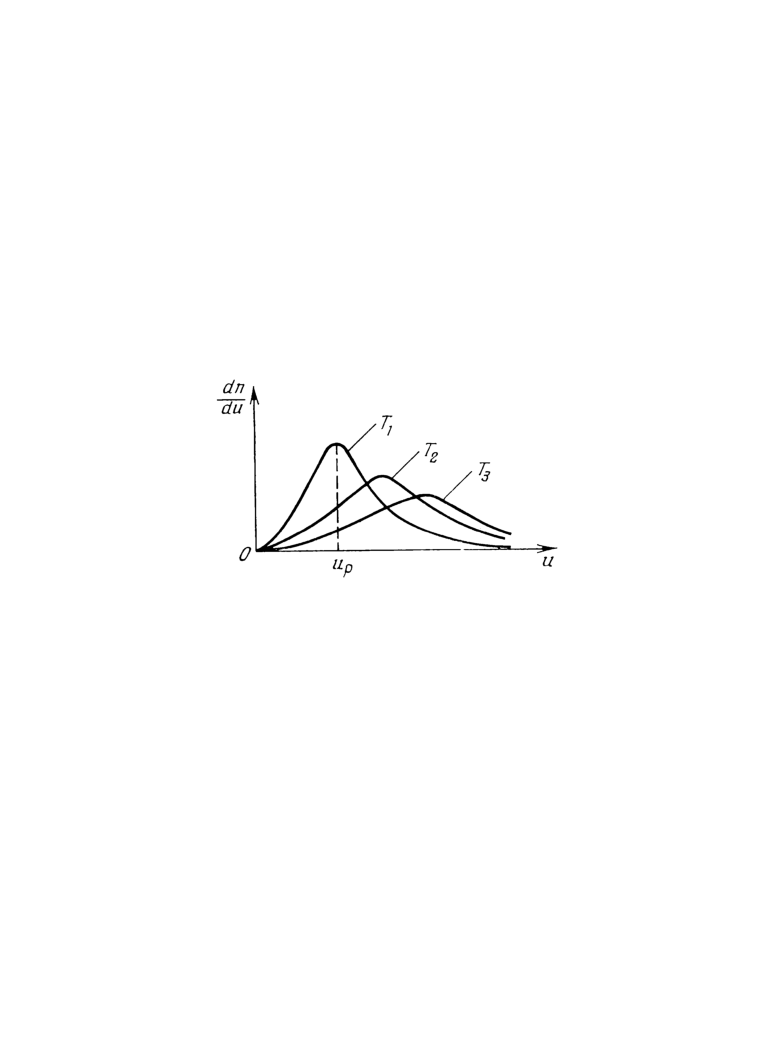
\includegraphics[width=0.8\textwidth]{figs/ch-10/fig-10-02.pdf}
%\input{figs/ch-03/fig-03-01}
%  \vspace{-13pt}
\sidecaption{Molecular velocity distribution for various temperatures.\zhcap{不同温度下的分子速率分布。}\label{fig-10-2}}
\end{figure}


\subsection{}\label{10.3.3} Another form of the Maxwellian distribution is
\zhpar{麦克斯韦分布的另一种形式为}
\begin{equation*}%
\dd n =n_{0} \left(\frac{m}{2 \pi k T}\right)^{3/2} \exp \left( - \frac{mu^{2}}{2kT}\right) \dd u_{x} \dd u_{y} \dd u_{z},
\end{equation*}
where $u_{x}$, $u_{y}$ and $u_{z}$ are projections of the molecular velocity on the coordinate axes. Owing to the random nature of thermal motion of the molecules \ssect{8.1.1}, distributions of the molecules according to the projections $u_{i}$ of their velocities on the coor­dinate axes $(i = x, y, z)$ are mutually independent. Hence
\zhpar{式中 $u_{x}$、$u_{y}$ 和 $u_{z}$ 为分子速度在各坐标轴上的投影。由于分子热运动的无规则性 \ssect{8.1.1}，分子速度在各坐标轴上投影 $u_{i}$（$i = x, y, z$）的分布彼此独立。因此}
\begin{equation*}%
\dd n= n_{0} f(u_{x}) \,f(u_{y}) \,f(u_{z}) \dd u_{x} \dd u_{y} \dd u_{z},
\end{equation*}
 where
\zhpar{式中，}
\begin{equation*}%
f(u_{i}) = \left(\frac{m}{2 \pi k T}\right)^{3/2} \exp \left( - \frac{mu_{i}^{2}}{2kT}\right)\quad (i =x,\,y,\,z),
\end{equation*}
is a distribution function of the projections of the molecular velocities.
\zhpar{是分子速度投影的分布函数。}

The Maxwellian distribution is isotropic. This is evident from the fact that the function $f(u_{x}, u_{y}, u_{z})$ depends only upon the speed (magnitude of the velocity), and because the function  $f(u_{i})$ is the same along all the axes.
\zhpar{麦克斯韦分布是各向同性的。这一点可由以下事实看出：函数 $f(u_{x}, u_{y}, u_{z})$ 只依赖于速率（速度的大小），而函数 $f(u_{i})$ 沿各坐标轴的形式相同。}

\subsection{}\label{10.3.4} The law of the distribution of molecular velocities \ssect{10.3.2} can be used to determine the \redem{most probable velocity} $u_{\textrm{p}}$ of the molecules, which corresponds to the maximum of the function
\zhpar{利用分子速率分布律 \ssect{10.3.2}，可以确定分子的\redem{最概然速率} $u_{\textrm{p}}$，它对应于下列函数的极大值：}
\begin{equation*}%
f(u) = \dv{n}{u} = 4 \pi n_{0} \left( \frac{m}{4 \pi k T} \right)^{1/2} \exp \left(- \frac{mu^{2}}{2kT} \right).
\end{equation*}
The condition 
\zhpar{上述极值条件为}
\begin{equation*}%
\left[ \dv{u} \left( \exp \left(- \frac{mu^{2}}{2kT} \right) u^{2} \right)
 \right]_{u=u_{\textrm{p}}} = 0,
\end{equation*}
yields
\zhpar{由此得到}
\begin{equation*}%
u_{\textrm{p}} = \sqrt{\frac{2kT}{m}}= \sqrt{\frac{2RT}{\mu}} = v_{\textrm{rms}} \sqrt{\frac{2}{3}}.
\end{equation*}

\subsection{}\label{10.3.5} A third form of the law of the distribution of molecular velocities is
\zhpar{分子速率分布律的第三种形式为}
\begin{equation*}%
\dd n = \frac{4 n_{0}}{\sqrt{\pi}} \exp \left( - \frac{u^{2}}{u_{\textrm{p}^{2}}}\right) \left( \frac{u}{u_{\textrm{p}}}\right)^{2} \dv{u}{u_{\textrm{p}}}.
\end{equation*}
The fraction $\dd n/n_{0}$ of the molecules of a gas having velocities lying within the range from $u$ to $u + \dd u$ is numerically equal to the hatched area $\dd S$ under the curve in \figr{fig-10-03}, which represents the dependence of $(u_{\textrm{p}}/n_{0}) \,(\dd n/\dd u)$ on $u/u_{\textrm{p}}$:
\zhpar{气体分子中速率位于 $u$ 到 $u + \dd u$ 范围内的分子所占比例 $\dd n/n_{0}$，在数值上等于\figr{fig-10-03} 中曲线下的阴影面积 $\dd S$。该曲线表示 $(u_{\textrm{p}}/n_{0}) \,(\dd n/\dd u)$ 随 $u/u_{\textrm{p}}$ 的变化关系，即：}
\begin{equation*}%
\dd S = \left( \frac{u_{\textrm{p}}}{n_{0}}\, \dv{n}{u} \right) \frac{\dd u}{u_{\textrm{p}}} = \frac{\dd n}{n_{0}}.
\end{equation*}
The area under the curve in \figr{fig-10-03}, i.e. bounded by the curve and the axis of abscissas, is equal to unity. This area represents the fraction of the molecules having all possible velocity values from 0 to $\infty$.
\zhpar{曲线与横坐标轴所围成的面积等于 1。该面积表示速率取值从 0 到 $\infty$ 的全部分子所占的比例。}
\begin{marginfigure}%[!ht]
%\begin{wrapfigure}{r}{0.5\linewidth}
\centering
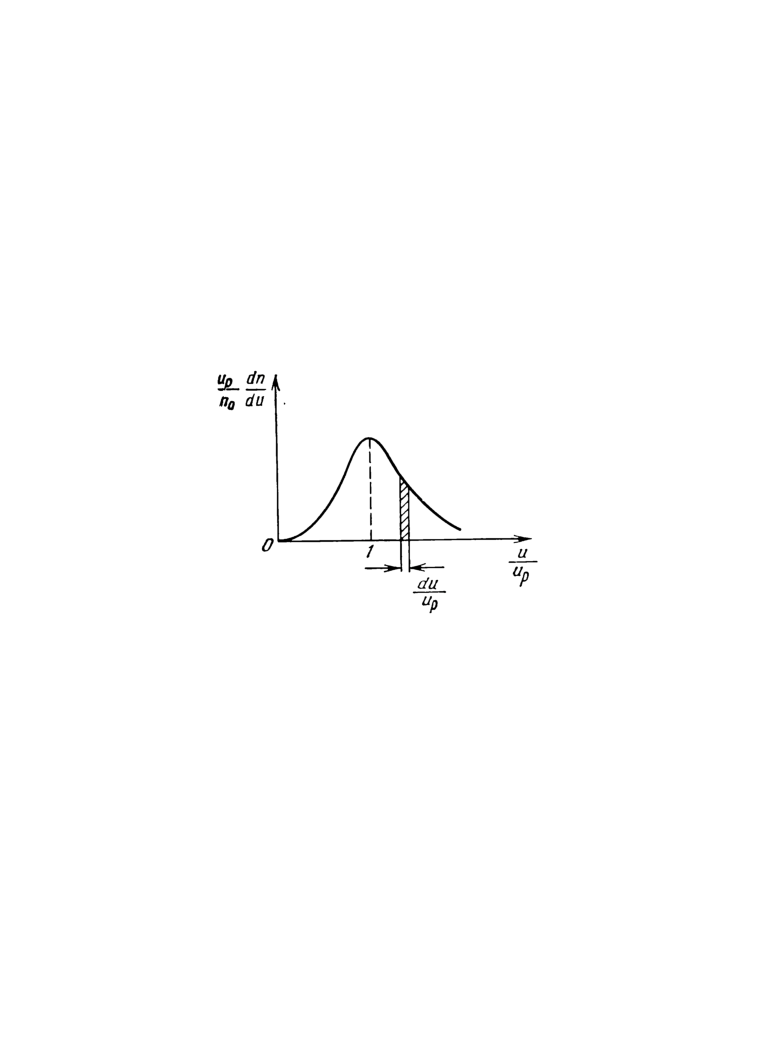
\includegraphics[width=\textwidth]{figs/ch-10/fig-10-03.pdf}
%\input{figs/ch-03/fig-03-01}
%  \vspace{-13pt}
\sidecaption{A velocity distribution curve for molecules.\zhcap{分子的速率分布曲线。}
\label{fig-10-03}}
\end{marginfigure}

\subsection{}\label{10.3.6} The arithmetic mean velocity $\expval{u}$ of translational motion of the molecules in an ideal gas, calculated by means of the distribution law \ssect{10.3.2}, is
\zhpar{理想气体中分子平动的算术平均速率 $\expval{u}$，利用分布律 \ssect{10.3.2} 计算，为}
\begin{equation*}%
\expval{u} = v_{\textrm{rms}} \sqrt{\frac{8}{3 \pi}} = \sqrt{\frac{8RT}{\pi \mu }} = \sqrt{\frac{8kT}{\pi m }} = 1.60 \sqrt{pv}.
\end{equation*}


\subsection{}\label{10.3.7} The energy distribution of the molecules in an ideal gas determines the fraction $\dd n_{E^{m}}/n_{0}$ of molecules, of their total number $n_{0}$, having kinetic energies $E_{k}^{\textrm{m}}= mu^{2}/2$ lying within the range from $E_{k}^{\textrm{m}} \qq{to} E_{k}^{\textrm{m}} + \dd E_{k}^{\textrm{m}}$:
\zhpar{理想气体分子的能量分布决定了动能 $E_{k}^{\textrm{m}}= mu^{2}/2$ 位于 $E_{k}^{\textrm{m}}$ 到 $E_{k}^{\textrm{m}} + \dd E_{k}^{\textrm{m}}$ 范围内的分子占其总数 $n_{0}$ 的比例 $\dd n_{E^{m}}/n_{0}$：}
\begin{equation*}%
\dd n_{E^{m}} = \frac{2 n_{0}}{\sqrt{\pi}} \left( kT \right)^{-3/2} \, \exp \left( -\frac{E_{k}^{\textrm{m}}}{kT} \right) \sqrt{E_{k}^{\textrm{m}}} \dd E_{k}^{\textrm{m}}.
\end{equation*}
Here $\dd n_{E^{m}}/n_{0} = f (E_{k}^{\textrm{m}} ) \,\dd E_{k}^{\textrm{m}}$, where $f(E_{k}^{\textrm{m}})$ is the distribution function for the molecular energies in an ideal gas. 
\zhpar{此处 $\dd n_{E^{m}}/n_{0} = f (E_{k}^{\textrm{m}} ) \,\dd E_{k}^{\textrm{m}}$，其中 $f(E_{k}^{\textrm{m}})$ 为理想气体中分子能量的分布函数。}

\hlblue{Example.} The average kinetic energy $\expval{E_{k}^{\textrm{m}}}$ of a molecule in an ideal gas is
\zhpar{\hlblue{例：}理想气体中分子的平均动能 $\expval{E_{k}^{\textrm{m}}}$ 为}
\begin{align*}%
\expval{E_{k}^{\textrm{m}}} & = \int_{0}^{\infty} E_{k}^{\textrm{m}} \, f(E_{k}^{\textrm{m}}) \, \dd E_{k}^{\textrm{m}} \\
& = \frac{2}{\sqrt{\pi} (kT)^{3/2}} \int_{0}^{\infty} E_{k}^{\textrm{m}} \exp \left(- \frac{E_{k}^{\textrm{m}}}{kT} \right) \sqrt{E_{k}^{\textrm{m}}} \dd E_{k}^{\textrm{m}}\\
& = \frac{3}{2} kT.
\end{align*}

(cf. \ssect{10.2.4}).
\zhpar{（参见 \ssect{10.2.4}）。}

\subsection{}\label{10.3.8} The relative motion \ssect{7.1.2} of two particles with the masses $m_{1}$ and $m_{2}$ is equivalent to the motion of a single particle with the reduced mass $m_{\textrm{red}} = m_{1}m_{2}/(m_{1}+ m_{2})$. For a homo­geneous gas $m_{1}= m_{2}= m$ and $m_{\textrm{red}} = m/2$. The distribution of molecules according to their relative velocities establishes the fraction $\dd n_{u_{\textrm{rel}}}/n_{0}$ of molecules, of their total number $n_{0}$,
having relative velocities $u_{\textrm{rel}}$ lying within the range from $u_{\textrm{rel}}$  to $u_{\textrm{rel}} + \dd u_{\textrm{rel}}$:
\zhpar{质量分别为 $m_{1}$ 和 $m_{2}$ 的两个粒子的相对运动，等效于一个约化质量为 $m_{\textrm{red}} = m_{1}m_{2}/(m_{1}+ m_{2})$ 的单个粒子的运动 \ssect{7.1.2}。对于均匀气体，$m_{1}= m_{2}= m$，$m_{\textrm{red}} = m/2$。按相对速度对分子进行分布，可以确定相对速率 $u_{\textrm{rel}}$ 位于 $u_{\textrm{rel}}$ 到 $u_{\textrm{rel}} + \dd u_{\textrm{rel}}$ 范围内的分子占其总数 $n_{0}$ 的比例 $\dd n_{u_{\textrm{rel}}}/n_{0}$：}
\begin{equation*}%
\dd n_{u_{\textrm{rel}}} = n_{0} \left( \frac{m}{4 \pi kT}\right)^{3/2} \exp \left(- \frac{mu^{2}_{\textrm{rel}}}{4kT} \right) 4 \pi u^{2}_{\textrm{rel}} \dd u_{\textrm{rel}}.
\end{equation*}
Here $\dd n_{u_{\textrm{rel}}} / n_{0}= f(u_{\textrm{rel}}) \dd u_{\textrm{rel}}$, where 
\zhpar{此处 $\dd n_{u_{\textrm{rel}}} / n_{0}= f(u_{\textrm{rel}}) \dd u_{\textrm{rel}}$，其中 $f(u_{\textrm{rel}})$ 的表达式为}
\begin{equation*}%
f(u_{\textrm{rel}}) = 4 \pi \left( \frac{m}{4 \pi kT} \right)^{3/2}\exp \left(- \frac{m u^{2}_{\textrm{rel}}}{4kT} \right) u_{\textrm{rel}}^{2},
\end{equation*}
is the relative velocity distribution of the molecules in an ideal gas.
\zhpar{为理想气体中分子的相对速率分布函数。}

\hlblue{Example.} The \redem{average relative velocity} $\expval{u_{\textrm{rel}}}$ of the mole­cules is
\zhpar{\hlblue{例：}分子的\redem{平均相对速率} $\expval{u_{\textrm{rel}}}$ 为}
\begin{equation*}%
\expval{u_{\textrm{rel}}} = \int_{0}^{\infty} u_{\textrm{rel}} f(u_{\textrm{rel}}) \, \dd u_{\textrm{rel}} = \sqrt{2} \sqrt{\frac{8kT}{\pi m}} = \sqrt{2} \expval{u},
\end{equation*}
where $\expval{u}$ is the arithmetic mean velocity of the molecules \ssect{10.3.6}.
\zhpar{式中 $\expval{u}$ 为分子的算术平均速率 \ssect{10.3.6}。}


\section[Boltzmann Distribution]{Particle Distribution in a Potential Force Field (Boltzmann Distribution)}
\label{sec-10.4}
\zhtitle{势力场中的粒子分布（玻尔兹曼分布）}


\subsection{}\label{10.4.1} 
Gases are ordinarily in the potential (conservative) gravitational fields of the earth \ssect{6.2.1}. If there were no such gravitational field, the atmospheric air would be dispersed in the universe. If, on the other hand, there were no thermal motion, the molecules of atmospheric air would drop to the earth. Gravity and thermal motion lead to a steady state of gases, in which their concentration and pressure decrease with an increase of their altitude above the earth's surface.
\zhpar{气体通常处于地球的势（保守）引力场中 \ssect{6.2.1}。若没有这样的引力场，大气就会弥散到宇宙中；若没有热运动，大气分子则会全部落到地面上。引力与热运动共同作用，使气体达到稳定状态：其浓度和压强随离地面高度的增加而减小。}

\subsection{}\label{10.4.2} If a gas (or other system of particles) is located in an external potential (conservative) force field \ssect{3.1.6}, the distri­bution of the particles throughout the volume is described by the \redem{Boltzmann distribution law}. This law establishes the number of particles $\dd n (x, \,y, \,z)$ that have coordinates within the ranges from $x$ to $x+ \dd x$, from $y$ to $y+ \dd y$, and from $z$ to $z+ \dd z$. In other words, $\dd n (x, \, y, \, z)$ is the number of molecules contained in the element of volume $\dd V = \dd x \dd y \dd z$. The Boltzmann distribution law is of the form
\zhpar{若气体（或其他粒子系统）处于外部势（保守）力场 \ssect{3.1.6} 中，粒子在整个体积内的分布由\redem{玻尔兹曼分布律}描述。该定律给出坐标分别位于 $x$ 到 $x+ \dd x$、$y$ 到 $y+ \dd y$ 以及 $z$ 到 $z+ \dd z$ 范围内的粒子数 $\dd n (x, \,y, \,z)$。换言之，$\dd n (x, \, y, \, z)$ 是包含在体积元 $\dd V = \dd x \dd y \dd z$ 中的分子数。玻尔兹曼分布律的形式为}
\begin{equation*}%
\dd n \, (x, \,y, \,z)= \textrm{const}\,\, \exp \left( -\frac{E_{\text{p}}^{\textrm{m}}}{kT}\right) \, \dd x \, \dd y \, \dd z,
\end{equation*}
where $E_{\textrm{p}}^{\textrm{m}}(x, \,y,\, z)$ is the potential energy of a particle in the external force field, $k$ is Boltzmann's constant, and $T$ is the absolute temperature. The value of the constant in the preceding equation is determined from the normalization condition:
\zhpar{式中 $E_{\textrm{p}}^{\textrm{m}}(x, \,y,\, z)$ 为粒子在外力场中的势能，$k$ 为玻尔兹曼常量，$T$ 为热力学温度。上式中的常数由归一化条件确定：}
\begin{equation*}%
\int \dd n = n_{0},
\end{equation*}
where $n_{0}$ is the total number of particles in unit volume.
\zhpar{式中 $n_{0}$ 为单位体积内粒子的总数。}


\hlblue{Example.} For particles of mass $m$, located in the earth's gravi­tational field, $E_{\textrm{p}}^{\text{m}}= mgh$ \ssect{3.3.3}, where $g$ is the acceleration due to gravity \ssect{7.3.3}, and $h$ is the altitude. At each altitude there is a Maxwellian molecular velocity distribution \ssect{10.3.1}. The number of molecules contained in the volume $\dd V$ is
\zhpar{\hlblue{例：}质量为 $m$ 的粒子处于地球引力场中时，$E_{\textrm{p}}^{\text{m}}= mgh$ \ssect{3.3.3}，其中 $g$ 为重力加速度 \ssect{7.3.3}，$h$ 为高度。在各高度上，分子速度都服从麦克斯韦分布 \ssect{10.3.1}。体积 $\dd V$ 内所含的分子数为}
\begin{equation*}%
\dd n \,(x, y, z) = \textrm{const} \exp\left( -\frac{mgh}{kT}\right) \dd V.
\end{equation*}
The gas density $\rho = m \dd n/ \dd V$ decreases with an increase in the altitude according to the exponential law 
\zhpar{气体密度 $\rho = m \dd n/ \dd V$ 随高度增加按指数律减小：}
\begin{equation*}%
\rho = \text{const} \exp\left( -\frac{mgh}{kT}\right).
\end{equation*}
The value of the constant can be determined from the condition $\rho = \rho_{0} = \text{const}$ at $h = 0$. The density of the gas or its pressure varies according to the \redem{barometric height formula}
\zhpar{由 $h = 0$ 时 $\rho = \rho_{0}$ 的条件可确定该常数的值。气体的密度或压强按\redem{气压高度公式}变化：}
\begin{equation*}%
\rho = \rho_{0} \exp\left( -\frac{mgh}{kT}\right) \qq{and} p = p_{0} \exp\left( -\frac{mgh}{kT}\right).
\end{equation*}

\subsection{}\label{10.4.3} The \redem{Maxwell-Boltzmann law}, or \redem{distribution}, describes the distribution of the coordinates and velocities of gas mole­ cules subject to the action of an arbitrary potential (conserva­ tive) force field:
\zhpar{描述气体分子在任意势（保守）力场作用下坐标和速度分布的是\redem{麦克斯韦-玻尔兹曼分布律}（或称\redem{分布}）：}
\begin{align*}%
\dd n & = \text{const} \exp\left( -\frac{p_{x}^{2}+p_{y}^{2}+p_{z}^{2}}{2mkT}\right) \dd p_{x} \dd p_{y} \dd p_{z}, \\
& \times \exp\left( -\frac{E_{\text{p}}^{\text{m}}(x,y,z)}{kT}\right)  \dd x \dd y \dd z.
\end{align*}
where $\dd n$ is the number of molecules contained in six-dimensio­nal space within the element of volume $\dd \Gamma=\dd x \dd y \dd z \, \dd p_{x} \dd p_{y} \dd p_{z}$, and $E_{\text{p}}^{\text{m}}(x,y,z)$ is the potential energy of a molecule in the external force field at a point with the coordinates $x$, $y$ and $z$, and the projections $p_{x}$, $p_{y}$ and $p_{z}$ of the momenta on the axes. The Maxwell-Boltzmann law is the product of two distribution functions. One of them describes the distribution with respect to coordinates, and the other with respect to momenta (or velocities).
\zhpar{式中 $\dd n$ 为六维空间中体积元 $\dd \Gamma=\dd x \dd y \dd z \, \dd p_{x} \dd p_{y} \dd p_{z}$ 内所包含的分子数，$E_{\text{p}}^{\text{m}}(x,y,z)$ 为分子在外力场中坐标为 $x$、$y$、$z$ 的点处的势能，$p_{x}$、$p_{y}$ 和 $p_{z}$ 为动量在各坐标轴上的投影。麦克斯韦-玻尔兹曼分布律是两个分布函数的乘积：其中一个描述对坐标的分布，另一个描述对动量（或速度）的分布。}


\section{Mean Free Path of Molecules}
\zhtitle{分子的平均自由程}


\subsection{}\label{10.5.1} Gas molecules have finite dimensions \ssect{8.4.1} and are continuously colliding with one another in thermal motion. Between two successive collisions, molecules travel at uniform velocity in a straight line over certain distances called their free paths $\lambda$. The mean free path $\expval{\lambda}$ is the average distance that a molecule travels without a collision. The mean free path is a characteristic of the whole totality of gas molecules at given values of $p$ and $T$.
\zhpar{气体分子具有有限的线度 \ssect{8.4.1}，并在热运动中不断地相互碰撞。在两次连续碰撞之间，分子沿直线做匀速运动，所经过的距离称为其自由程 $\lambda$。平均自由程 $\expval{\lambda}$ 是分子在两次碰撞之间经过的平均距离。平均自由程是在给定的 $p$ 和 $T$ 下，全体气体分子的特征量。}

\subsection{}\label{10.5.2} In unit time each molecule undergoes a mean number of collisions $\expval{z}$ (\redem{average collision frequency}) equal to
\zhpar{单位时间内每个分子的平均碰撞次数 $\expval{z}$（\redem{平均碰撞频率}）等于}
\begin{equation*}%
\expval{z^{2}} = \pi d^{2} n_{0} \expval{u_{\text{rel}}} = \sqrt{2} \pi d^{2} n_{0} \expval{u}.
\end{equation*}
Here $d$ is the effective diameter of the molecule \ssect{8.4.1}, $n_{0}$ is the number of molecules in unit volume of the gas, $\expval{u_{\text{rel}}}$ is their average relative velocity \ssect{10.3.8}, and $\expval{u}$ is their arithmetic mean velocity \ssect{10.3.6}.
\zhpar{式中 $d$ 为分子的有效直径 \ssect{8.4.1}，$n_{0}$ 为气体单位体积内的分子数，$\expval{u_{\text{rel}}}$ 为分子的平均相对速率 \ssect{10.3.8}，$\expval{u}$ 为分子的算术平均速率 \ssect{10.3.6}。}

\subsection{}\label{10.5.3} The average distance travelled by a molecule in unit time is numerically equal to $\expval{u}$. Therefore $\expval{u} = \expval{\lambda}\expval{z}$. The mean free path $\expval{\lambda}$ is
\zhpar{单位时间内分子所经过的平均距离在数值上等于 $\expval{u}$，因此 $\expval{u} = \expval{\lambda}\expval{z}$。平均自由程 $\expval{\lambda}$ 为}
\begin{equation*}%
\expval{\lambda} = \frac{\expval{u}}{\expval{z}} = \frac{1}{\sqrt{2} d^{2}n_{0}}.
\end{equation*}
At constant temperature, $n_{0}$ is proportional to the pressure p of the gas \ssect{8.4.5}. Hence, for a given gas the mean free path is inversely proportional to the pressure:
\zhpar{在温度不变时，$n_{0}$ 与气体压强 $p$ 成正比 \ssect{8.4.5}。因此，对于给定气体，平均自由程与压强成反比：}
\begin{equation*}%
p_{1} \expval{\lambda_{1}}  = p_{2} \expval{\lambda_{2}} = \text{const}.
\end{equation*}%
in which the subscripts 1 and 2 refer to two states of the gas. 
\zhpar{式中下标 1 和 2 分别表示气体的两个状态。}

\subsection{}\label{10.5.4} If molecules are ejected from some source of particles and a beam is formed by means of a diaphragm, the free path distribution law is valid for the molecules of the beam:
\zhpar{若分子从某一粒子源射出，并经光阑形成分子束，则束中分子满足自由程分布律：}
\begin{equation*}%
N = N_{0} \exp \left( -\frac{x}{\expval{\lambda}}\right).
\end{equation*}
where $N$ is the number of molecules in the beam that have travelled a distance $x$ without collisions, and $N_{0}$ is the number of molecules in the beam at $x = 0$, i.e. at the output of the diaphragm.
\zhpar{式中 $N$ 为束中走过距离 $x$ 而未发生碰撞的分子数，$N_{0}$ 为 $x = 0$ 处（即光阑出口处）束中的分子数。}



\section[Equipartition of Energy]{Principle of the Equipartition of Energy. Internal Energy of an Ideal Gas}
\zhtitle{能量均分原理。理想气体的内能}

\subsection{}\label{10.6.1} The \redem{number of degrees of freedom} of a body is the minimum number of coordinates (number of independent coordinates) that it is necessary to specify in order to completely determine the position of the body in space.
\zhpar{物体的\redem{自由度数}是完全确定物体在空间中位置所需的最少独立坐标数。}



A particle, for instance, travelling along one of the coordinate axes has a single degree of freedom. The same particle travelling in a plane has two degrees of freedom. The position of a par­ticle travelling freely in space is determined by three degrees of freedom: the coordinates $x$, $y$ and $z$. A rigid body \ssect{1.1.4} has six degrees of freedom: its position in space is determined by the three coordinates of its centre of mass \ssect{2.3.3}, two an­gles, $\theta$ and $\varphi$, determining the direction of a certain axis, fixed in the body and passing through its centre of mass (\figr{fig-10-4}), and, in addition, angle $\psi$, determining the direction of a second axis, fixed in the body and perpendicular to the first axis. 
\zhpar{例如，沿某一坐标轴运动的质点具有一个自由度；在平面内运动的质点具有两个自由度；在空间中自由运动的质点，其位置由三个自由度（坐标 $x$、$y$ 和 $z$）确定。刚体 \ssect{1.1.4} 具有六个自由度：其在空间中的位置由以下几个量确定：质心 \ssect{2.3.3} 的三个坐标；两个角度 $\theta$ 和 $\varphi$，它们确定与刚体固连并通过质心的某一轴的方向（\figr{fig-10-4}）；以及角度 $\psi$，它确定与刚体固连且垂直于该轴的第二轴的方向。}
\begin{marginfigure}%[!ht]
%\begin{wrapfigure}{r}{0.5\linewidth}
\centering
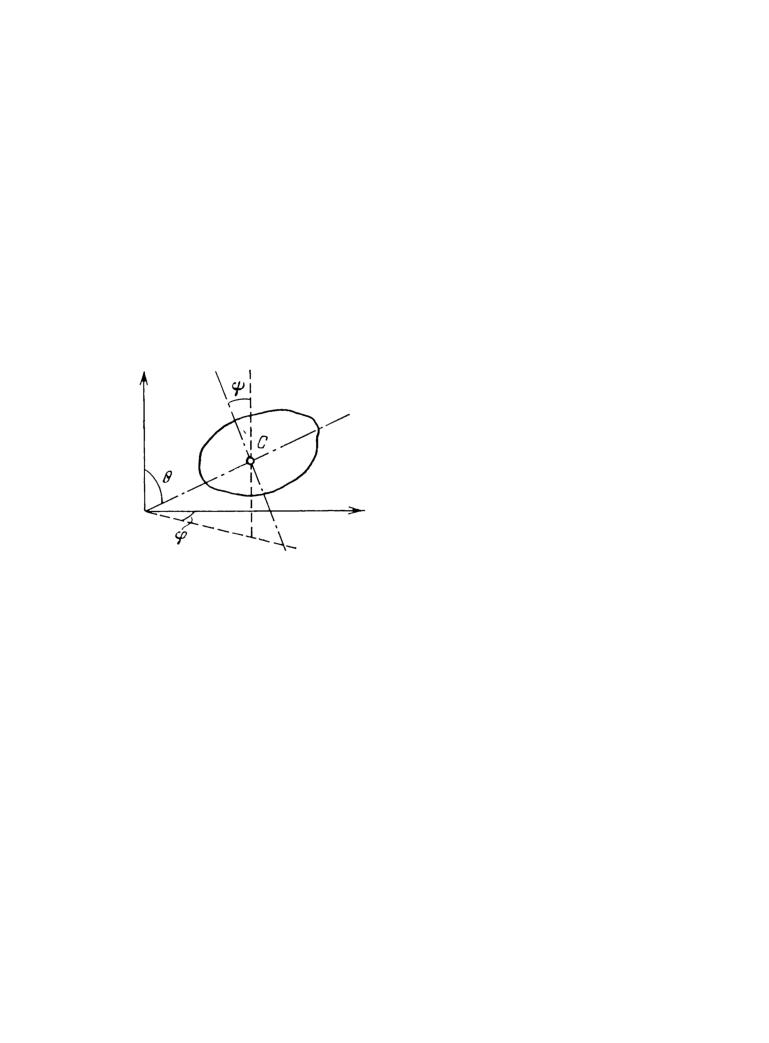
\includegraphics[width=0.8\textwidth]{figs/ch-10/fig-10-04.pdf}
%\input{figs/ch-03/fig-03-01}
%  \vspace{-13pt}
\sidecaption{Degrees of freedom for a particle.\zhcap{质点的自由度。}\label{fig-10-4}}
\end{marginfigure}

Changes in the three coordinates of the centre of mass at given constant angles $\theta$, $\varphi$ and $\psi$ correspond to translational motion of the rigid body. The coordinates of the centre of mass are the three degrees of freedom of translational motion. Changes in the angle $\theta$, $\varphi$ or $\psi$ at a constant position of the centre of mass lead to rotation of the rigid body. Hence, the correspond­ ing degrees of freedom are said to be rotary. Additional degrees of freedom of oscillatory, or vibratory, motion \ssect{10.6.5} are introduced to determine the position in space of an imperfectly rigid body, whose various parts can be displaced with respect to one another.
\zhpar{在质心的三个坐标变化而角度 $\theta$、$\varphi$ 和 $\psi$ 保持不变时，对应刚体的平动。质心的三个坐标即为平动的三个自由度。在质心位置不变、角度 $\theta$、$\varphi$ 或 $\psi$ 变化时，刚体发生转动，因此相应的自由度称为转动自由度。此外，为确定非完全刚性物体（其各部分可相对彼此位移）在空间中的位置，还需引入振动自由度 \ssect{10.6.5}。}


\subsection{}\label{10.6.2} In many problems a \redem{molecule of a monatomic gas} can be regarded as a particle (cf. \ssect{8.4.1}). This is based on the fact that practically all the mass of such an atom is concentrated in its nucleus \ssect{42.1.1}, which is of extremely small size. The molecule of monatomic gas has three degrees of freedom of translational motion. Its average kinetic energy $\expval{E_{\text{k}}^{\text{m}}}$ is equal to the kinetic energy of molecules travelling at a velocity equal to the root-mean-square velocity $v_{\text{rms}}$ \ssect{10.2.4}:
\zhpar{在许多问题中，\redem{单原子气体分子}可以视为质点（参见 \ssect{8.4.1}）。这是因为这种原子的几乎全部质量都集中在体积极小的原子核 \ssect{42.1.1} 中。单原子气体分子具有三个平动自由度。其平均动能 $\expval{E_{\text{k}}^{\text{m}}}$ 等于速率为方均根速率 $v_{\text{rms}}$ \ssect{10.2.4} 的分子的动能：}
\begin{equation*}%
\expval{E_{\text{k}}^{\text{m}}} = \frac{3}{2} k T.
\end{equation*}
Owing to the random nature of thermal motion of the mole­cules, this energy is uniformly distributed between the three degrees of freedom. Hence, on an average each degree of free­dom of translational motion of a monatomic molecule accounts
for the same amount of kinetic energy $ \expval{E_{\text{k}_{0}}^{\text{m}}} = \expval{E_{\text{k}}^{\text{m}}}/3 = kT/2 $, where $k$ is Boltzmann's constant and $T$ is the absolute temperature.
\zhpar{由于分子热运动的无规则性，该能量在三个自由度之间均匀分布。因此，平均而言，单原子分子的每个平动自由度所具有的动能相同，都为 $ \expval{E_{\text{k}_{0}}^{\text{m}}} = \expval{E_{\text{k}}^{\text{m}}}/3 = kT/2 $，式中 $k$ 为玻尔兹曼常量，$T$ 为热力学温度。}

\begin{marginfigure}%[!ht]
%\begin{wrapfigure}{r}{0.5\linewidth}
\centering
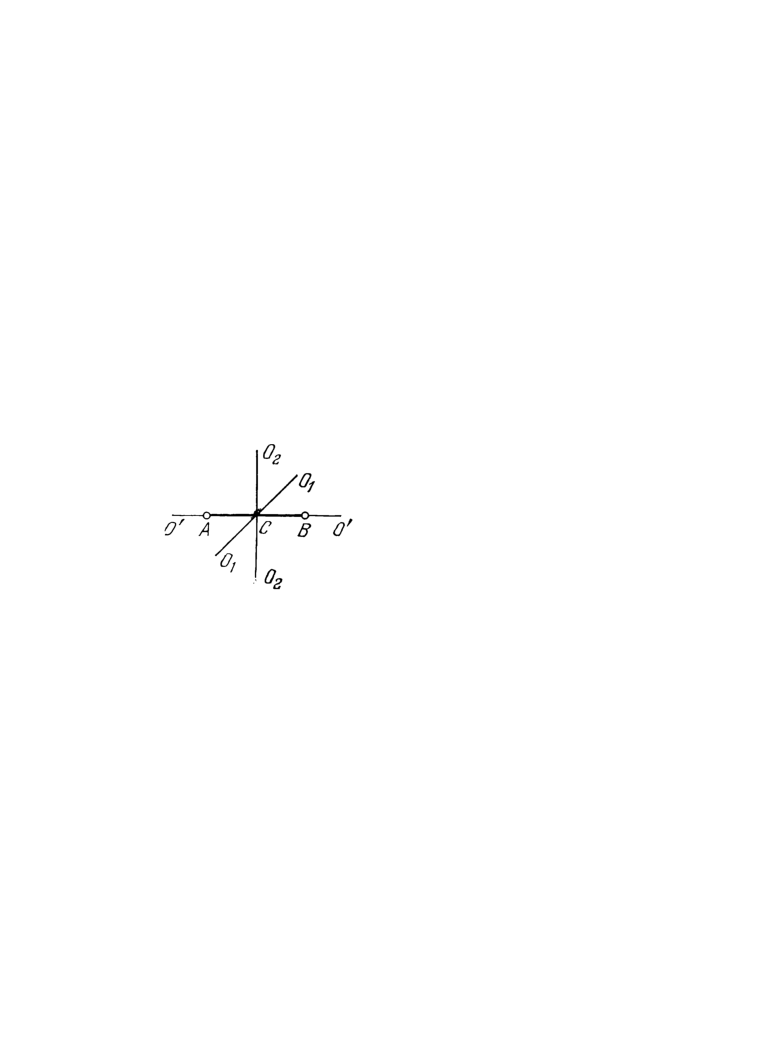
\includegraphics[width=0.8\textwidth]{figs/ch-10/fig-10-05.pdf}
%\input{figs/ch-03/fig-03-01}
%  \vspace{-13pt}
\sidecaption{Degrees of freedom of A diatomic molecule.\zhcap{双原子分子的自由度。}\label{fig-10-5}}
\end{marginfigure}


\subsection{}\label{10.6.3} As a first approximation, a molecule of a diatomic gas consists of two atoms, $A$ and $B$, rigidly held together by an incompressible, undeformable bond (\figr{fig-10-5}). In addition to the three degrees of freedom of translational motion, the centre of mass $C$ \ssect{2.3.3} of such a molecule has two more degrees of freedom of rotary motion about axes $O_{1}-O_{1}$ and $O_{2}-O_{2}$. Rota­tion about the third axis $O'-O'$ makes no contribution to the molecule's energy because the moment of inertia \ssect{4.2.1} of the atoms with respect to this axis is negligibly small. Thus, a diatomic molecule has five degrees of freedom. Molecules consisting of three or more atoms have six degrees of freedom: three translational and three rotary degrees (\figr{fig-10-6}). 
\zhpar{作为第一近似，双原子气体分子可视为两个原子 $A$ 和 $B$ 通过不可压缩、不可形变的键刚性地结合在一起（\figr{fig-10-5}）。除三个平动自由度外，分子质心 $C$ \ssect{2.3.3} 还具有两个绕轴 $O_{1}-O_{1}$ 和 $O_{2}-O_{2}$ 转动的转动自由度。绕第三轴 $O'-O'$ 的转动对分子能量没有贡献，因为两原子相对该轴的转动惯量 \ssect{4.2.1} 可以忽略不计。因此，双原子分子具有五个自由度。由三个或更多原子组成的分子具有六个自由度：三个平动自由度和三个转动自由度（\figr{fig-10-6}）。}

\begin{marginfigure}%[!ht]
%\begin{wrapfigure}{r}{0.5\linewidth}
\centering
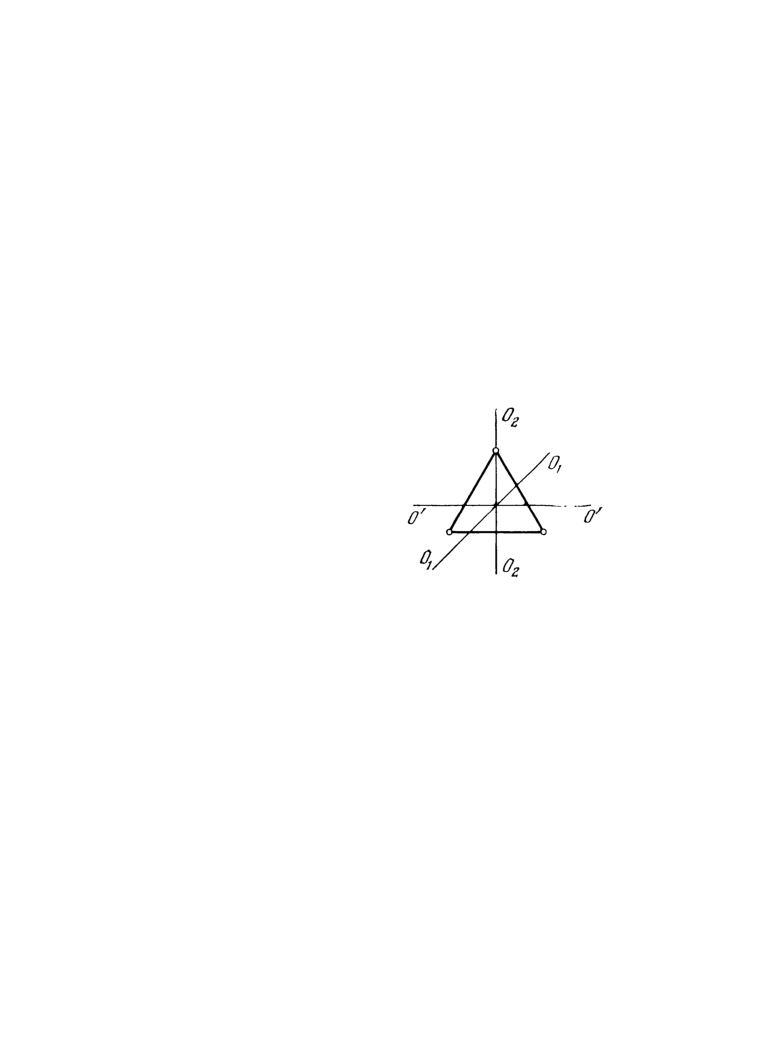
\includegraphics[width=0.8\textwidth]{figs/ch-10/fig-10-06.pdf}
%\input{figs/ch-03/fig-03-01}
%  \vspace{-13pt}
\caption{Degrees of freedom of molecules with three or more atoms.\zhcap{由三个或更多原子组成的分子的自由度。}\label{fig-10-6}}
\end{marginfigure}

\subsection{}\label{10.6.4} The principle of equipartition of energy states that on an average each degree of freedom of a molecule accounts for the same amount of kinetic energy, equal to $kT/2.$ If a mol­ecule has $i$ degrees of freedom its average kinetic energy $\expval{E_{\text{k}}^{\text{m}}}= ikT/2$.
\zhpar{能量均分原理指出：平均而言，分子的每个自由度所对应的动能都相同，均为 $kT/2$。若分子具有 $i$ 个自由度，则其平均动能为 $\expval{E_{\text{k}}^{\text{m}}}= ikT/2$。}

The principle of equipartition of energy leads to the conclusion that all degrees of freedom of the molecule are equally justified: each makes the same contribution to its average energy. This conclusion actually has only a limited field of application, and has been revised for quantum statistics \ssect{41.1.1}.
\zhpar{能量均分原理表明，分子的所有自由度地位平等，每个自由度对其平均能量的贡献都相同。这一结论实际上只有有限的适用范围，在量子统计中已作了修正 \ssect{41.1.1}。}

\subsection{}\label{10.6.5} In real molecules, which are not absolutely rigid, vibra­tory degrees of freedom make a contribution to the energy of the molecule in accordance with the principle of equipartition of energy \ssect{10.6.4}. Each vibratory degree of freedom accounts, not only for kinetic energy $\expval{E_{\text{k}}^{\text{m}}}$ but for potential energy $\expval{E_{\text{p}}^{\text{m}}}$ as well. For harmonic vibrations \ssect{28.1.3}, $\expval{E_{\text{k}_{0}}^{\text{m}}} = \expval{E_{\text{p}_{0}}^{\text{m}}}$. According to \ssect{10.6.4}
\zhpar{在真实分子中，原子之间并非绝对刚性，振动自由度依照能量均分原理对分子能量有所贡献 \ssect{10.6.4}。每个振动自由度不仅对动能 $\expval{E_{\text{k}}^{\text{m}}}$ 有贡献，也对势能 $\expval{E_{\text{p}}^{\text{m}}}$ 有贡献。对于简谐振动 \ssect{28.1.3}，有 $\expval{E_{\text{k}_{0}}^{\text{m}}} = \expval{E_{\text{p}_{0}}^{\text{m}}}$。根据 \ssect{10.6.4}，有}
\begin{equation*}%
\expval{E_{\text{k}_{0}}^{\text{m}}} = \expval{E_{\text{p}_{0}}^{\text{m}}}  = \frac{1}{2}kT,
\end{equation*}
where $\expval{E_{\text{k}_{0}}^{\text{m}}}$ and $\expval{E_{\text{p}_{0}}^{\text{m}}}$ are the average kinetic and potential energies of a molecule per vibratory degree of freedom.
\zhpar{式中 $\expval{E_{\text{k}_{0}}^{\text{m}}}$ 和 $\expval{E_{\text{p}_{0}}^{\text{m}}}$ 分别为分子每个振动自由度的平均动能和平均势能。}

The average value $\expval{E_{0}^{\text{m}}}$ of the total energy of a molecule per vibratory degree of freedom is
\zhpar{分子每个振动自由度的总能量平均值 $\expval{E_{0}^{\text{m}}}$ 为}
\begin{equation*}%
\expval{E_{0}^{\text{m}}} = \expval{E_{\text{k}_{0}}^{\text{m}}} + \expval{E_{\text{p}_{0}}^{\text{m}}} = 2 \expval{E_{\text{k}_{0}}^{\text{m}}} = kT.
\end{equation*}
This equation is valid for harmonic vibrations of particles (atoms, molecules or ions) in the crystal lattice sites of sol­ids \ssect{8.1.4}.
\zhpar{该式适用于固体晶格格点上粒子（原子、分子或离子）的简谐振动 \ssect{8.1.4}。}

\subsection{}\label{10.6.6} The internal energy \ssect{9.1.2} of a polyatomic gas consti­tutes the kinetic energy of all kinds of motion of its particles. For one mole of such a gas
\zhpar{多原子气体的内能 \ssect{9.1.2} 由其粒子所有各种运动的动能构成。对于 1 摩尔此类气体，}
\begin{equation*}%
U = \expval{E_{\text{k}}^{\text{m}}} N_{A}= \frac{i}{2} k N_{A}T = i \frac{RT}{2},
\end{equation*}
where $N_{A}$ is Avogadro's number (Appendix~II), $i$ is the number of degrees of freedom of the molecule \ssect{10.6.4}, and $R$ is the universal gas constant \ssect{8.4.4}.
\zhpar{式中 $N_{A}$ 为阿伏伽德罗常量（见附录 II），$i$ 为分子的自由度数 \ssect{10.6.4}，$R$ 为摩尔气体常量 \ssect{8.4.4}。}


\section[Heat Capacity of Gases]{Heat Capacity of Monatomic, Diatomic and Polyatomic Gases}
\zhtitle{单原子、双原子和多原子气体的热容}

\subsection{}\label{10.7.1} The molecules of a monatomic gas have three degrees of freedom \ssect{10.6.2} and, according to\ssect{10.6.6}, the inter­nal energy of one mole of such a gas is $U = 3kN_{A}T/2$.
\zhpar{单原子气体分子具有三个自由度 \ssect{10.6.2}，根据 \ssect{10.6.6}，此类气体 1 摩尔的内能为 $U = 3kN_{A}T/2$。}

The molar heat capacity of such a gas at constant volume \ssect{9.5.4} is
\zhpar{此类气体在定容下的摩尔热容 \ssect{9.5.4} 为}
\begin{align*}%
C_{V\mu} & = \dv{U}{T} =\frac{3}{2} N_{A} k = \frac{3}{2} R \\
& = 1246.5 \frac{\si{\joule}}{\si{\mole\kelvin}} \\
& \approx 3  \frac{\si{\calorie}}{\si{\mole\kelvin}}\qq{because} R \approx 2  \frac{\si{\calorie}}{\si{\mole\kelvin}}.
\end{align*}
For a polyatomic gas whose molecules have $i$ degrees of freedom
\zhpar{对于分子具有 $i$ 个自由度的多原子气体，}
\begin{align*}%
C_{V\mu} & = \frac{iR}{2} = 4.16 i \frac{\si{\joule}}{\si{\mole\kelvin}} \\
& \approx i  \frac{\si{\calorie}}{\si{\mole\kelvin}}.
\end{align*}

\subsection{}\label{10.7.2} The molar heat capacity $C_{p\mu}$ at constant pressure (\ssect{9.5.7} and \ssect{9.5.8}) of a gas whose molecules have $i$ degrees of freedom is
\zhpar{分子具有 $i$ 个自由度的气体在定压下的摩尔热容 $C_{p\mu}$（见 \ssect{9.5.7} 和 \ssect{9.5.8}）为}
\begin{align*}%
C_{p\mu} & = \frac{(i+2)R}{2} = 4.16 (i+2) \frac{\si{\joule}}{\si{\mole\kelvin}}, \\
& \approx (i+2) \frac{\si{\calorie}}{\si{\mole\kelvin}}.
\end{align*}The principle of equipartition of energy \ssect{10.6.4} leads to the conclusion that the heat capacity of a gas depends upon the number of degrees of freedom of its molecules, but does not depend on the temperature. Experimental data disprove these conclusions of the classical theory of heat capacity. Investigations indicate that the heat capacity of gases increases and decreases with temperature.
\zhpar{能量均分原理 \ssect{10.6.4} 得出的结论是：气体的热容取决于其分子的自由度数，而与温度无关。实验数据否定了经典热容理论的这些结论。研究表明，气体的热容随温度的变化既有增大，也有减小。}

\subsection{}\label{10.7.3} A theoretical explanation of experimental data on the dependence of heat capacity on temperature in a wide tem­perature range is given in the quantum theory of heat capacity. This theory takes into account the following results obtained in a quantum-mechanical description of the properties of diatomic and polyatomic molecules:
\zhpar{在宽广的温度范围内，热容随温度变化的实验数据可由热容的量子理论给出理论解释。该理论考虑了用量子力学描述双原子和多原子分子性质时所得到的下列结果：}
\begin{enumerate}[label=(\alph*)]
\item Of the four parts that comprise the energy Em of the molecule \sidenote{This ignores the nuclear energy of the molecule, which has no influence on the heat capacity of molecules.} \ssect{39.5.2}, i.e.
\zhpar{在构成分子能量 $E^{\text{m}}$ 的四个部分中 \ssect{39.5.2}，即}
\zhpar{注：这里忽略了分子的核能，核能对分子热容没有影响。}
\begin{equation*}%
E^{\text{m}} = E_{t}^{\text{m}}+ E_{e}^{\text{m}} + E_{v}^{\text{m}} + E_{r}^{\text{m}},
\end{equation*}
only $E_{t}^{\text{m}}$ the energy of translational motion of the molecule's
centre of mass \ssect{2.3.3}, varies continuously (not by discrete amounts). The values of all other kinds of internal energy of molecules are quantized and thereby assume only a discrete series of values \ssect{39.4.5}. This refers to the following kinds of energy: $E_{e}^{\text{m}}$, the energy of motion of the electrons of the mole­cule; $E_{v}^{\text{m}}$, the energy of vibrational motion of the nuclei in the molecule; and $E_{r}^{\text{m}}$, the energy of rotary motion of the molecule. 
\zhpar{其中只有 $E_{t}^{\text{m}}$（分子质心平动的能量）是连续变化的，而不是按分立的量变化。分子内部其他各类能量的取值都是量子化的，因而只能取一系列分立值 \ssect{39.4.5}。这些能量包括：$E_{e}^{\text{m}}$，即分子中电子运动的能量；$E_{v}^{\text{m}}$，即分子中原子核振动的能量；$E_{r}^{\text{m}}$，即分子转动的能量。}

\item As a first approximation, the kinds of internal motion
of the molecule can be assumed independent of one another. Thus, at small amplitudes of vibration of the nuclei, the changes in the moments of inertia \ssect{4.2.1} of the molecule due to vibra­tion can be neglected, as can the effect of the vibrational motion in the molecule on its rotation.
\zhpar{作为第一近似，可以认为分子的各种内部运动彼此独立。因此，在原子核振幅较小时，可以忽略振动引起的分子转动惯量 \ssect{4.2.1} 的变化，也可以忽略分子振动对其转动的影响。}
\item No changes in the energy of motion of the electrons occur when a substance is heated by one degree at ordinary tempera­tures. Adjacent energy levels of the electrons in the molecule are separated by energy of the order of several $eV$, correspond­ ing to temperatures of several tens of thousands of degrees \ssect{10.7.6}. Therefore, the energy of motion of electrons in the molecule can be neglected in dealing with the heat capacities of monatomic and polyatomic gases up to the very highest temperatures.
\zhpar{在通常温度下，物质每升高一度，分子中电子的运动能量都不发生变化。分子中电子相邻能级的能量间隔为数个 $eV$ 的量级，相当于几万度的温度 \ssect{10.7.6}。因此，即使在最高温度下，计算单原子和多原子气体的热容时也可以忽略电子运动的能量。}
\end{enumerate}

\subsection{}\label{10.7.4} As a first approximation, the vibrational motion of the nuclei in the molecule is described as the vibration of a harmonic oscillator \ssect{38.5.4}, whose mass $m$ is equal to the reduced mass of a system of vibrating atoms, $m = m_{1}m_{2}/(m_{1} + m_{2})$, where $m_{1}$ and $m_{2}$ are the masses of the atoms. Then the energy of vibrational motion of the molecule equals 
\zhpar{作为第一近似，分子中原子核的振动可以描述为谐振子 \ssect{38.5.4} 的振动，其质量 $m$ 等于振动原子系统的约化质量 $m = m_{1}m_{2}/(m_{1} + m_{2})$，式中 $m_{1}$ 和 $m_{2}$ 为两原子的质量。于是，分子的振动能量为}
\begin{equation*}%
E_{v}^{\text{m}} = h \nu_{0} \left( n + \frac{1}{2}\right),
\end{equation*}
where $n$ is the quantum number and assumes integral values: $n = 0, \,1,\, 2, \ldots{}$, $\nu_{0}$ is the natural frequency of vibrations \ssect{38.5.5}, and $h$ is Planck's constant (Appendix~II). The energy of a harmonic oscillator, equal to $h\nu_{0}/2$ at $n = 0$, is conserved at any arbitrarily low temperatures, and even at $T \to 0$ \ssect{38.5.6}. The difference $\Delta E_{v}^{\text{m}}$ between the energies of two adjacent vibra­tional energy levels, $\Delta E_{v}^{\text{m}} = h\nu_{0}$, is independent of the quantum number. Valid at room and lower temperatures is the condi­tion: $\Delta E^{\text{m}}_{v} \gg kT$. No changes are observed in the energy of vibrational motion of molecules at such temperatures. In cal­culating the heat capacity of gases under such conditions, vibrational degrees of freedom of the molecule can be neglected. In the general case, vibrational motions make contributions to the internal energy $U_{v}$ \ssect{9.1.2} and the heat capacity $C_{V\mu}$ \ssect{9.5.2}. For one mole
\zhpar{式中 $n$ 为量子数，取整数值 $n = 0, \,1,\, 2, \ldots{}$，$\nu_{0}$ 为固有振动频率 \ssect{38.5.5}，$h$ 为普朗克常量（见附录 II）。谐振子在 $n = 0$ 时的能量为 $h\nu_{0}/2$，该能量在任意低的温度下，甚至在 $T \to 0$ 时都保持不变 \ssect{38.5.6}。相邻两个振动能级的能量差 $\Delta E_{v}^{\text{m}} = h\nu_{0}$ 与量子数无关。在室温及更低温度下，满足条件 $\Delta E^{\text{m}}_{v} \gg kT$。在这种温度下，分子的振动能量不发生变化，因此在计算此条件下的气体热容时，可以忽略分子的振动自由度。一般情况下，振动运动对内能 $U_{v}$ \ssect{9.1.2} 和热容 $C_{V\mu}$ \ssect{9.5.2} 都有贡献。对于 1 摩尔气体，}
\begin{align*}%
U_{v} & = \frac{N_{A}h \nu}{2} \frac{\left(\exp \left(\frac{h \nu}{2kT}\right) + \exp \left(-\frac{h \nu}{2kT}\right) \right)}{\left(\exp \left(\frac{h \nu}{2kT}\right) - \exp \left(-\frac{h \nu}{2kT}\right) \right)}, \\
C_{V\mu_{v}} & = \frac{N_{A}k}{4} \left(\frac{h \nu}{kT}\right)^{2} \left(\frac{\exp \left(\frac{h \nu}{2kT}\right) - \exp \left(-\frac{h \nu}{2kT}\right)}{2} \right)^{-2}.
\end{align*}
where $T$ is the absolute temperature, $k$ is Boltzmann's constant \ssect{8.4.5} and $N_{A}$ is Avogadro's number (Appendix~II). At high temperatures $(T \gg h\nu/k)$
\zhpar{式中 $T$ 为热力学温度，$k$ 为玻尔兹曼常量 \ssect{8.4.5}，$N_{A}$ 为阿伏伽德罗常量（见附录 II）。在高温条件 $(T \gg h\nu/k)$ 下，}
\begin{equation*}%
U_{v} \approx N_{A} k T = RT, \quad C_{V\mu v} \approx N_{A}k = R.
\end{equation*}
These results coincide with those of classical theory which follow from the principle of the equipartition of energy \ssect{10.6.4}. Under these conditions the energy of the oscillator can be assumed to vary continuously because $\Delta E^{m}_{v} \ll kT$. At sufficiently low temperatures $(T \ll h\nu/k)$
\zhpar{这些结果与由能量均分原理得出的经典理论结果一致 \ssect{10.6.4}。在这些条件下，由于 $\Delta E^{m}_{v} \ll kT$，可以认为振子的能量连续变化。在足够低的温度（$T \ll h\nu/k$）下，}
\begin{align*}%
U_{v} & \approx  \frac{N_{A}h \nu}{2} + N_{A}h \nu  \exp \left(-\frac{h \nu}{kT}\right),\\
C_{V\mu_{v}} & \approx N_{A}k \left(\frac{h \nu}{kT}\right)^{2}\exp \left(-\frac{h \nu}{kT}\right).
\end{align*}
As $T \to 0$, the energy $U_{v} \to N_{A} h \nu/2$. This quantity is called the \redem{zero-point vibrational energy} of the system \ssect{38.5.6}. As $T \to 0$, the heat capacity $C_{V\mu v} \to 0$ in accordance with the third law of thermodynamics \ssect{11.8.4}. The dependence $C_{V\mu v} = f(T)$ for diatomic gases is shown in \figr{fig-10-07}.
\zhpar{当 $T \to 0$ 时，能量 $U_{v} \to N_{A} h \nu/2$。该量称为体系的\redem{零点振动能} \ssect{38.5.6}。根据热力学第三定律 \ssect{11.8.4}，当 $T \to 0$ 时热容 $C_{V\mu v} \to 0$。双原子气体的 $C_{V\mu v} = f(T)$ 关系如 \figr{fig-10-07} 所示。}
\begin{marginfigure}%[!ht]
%\begin{wrapfigure}{r}{0.5\linewidth}
\centering
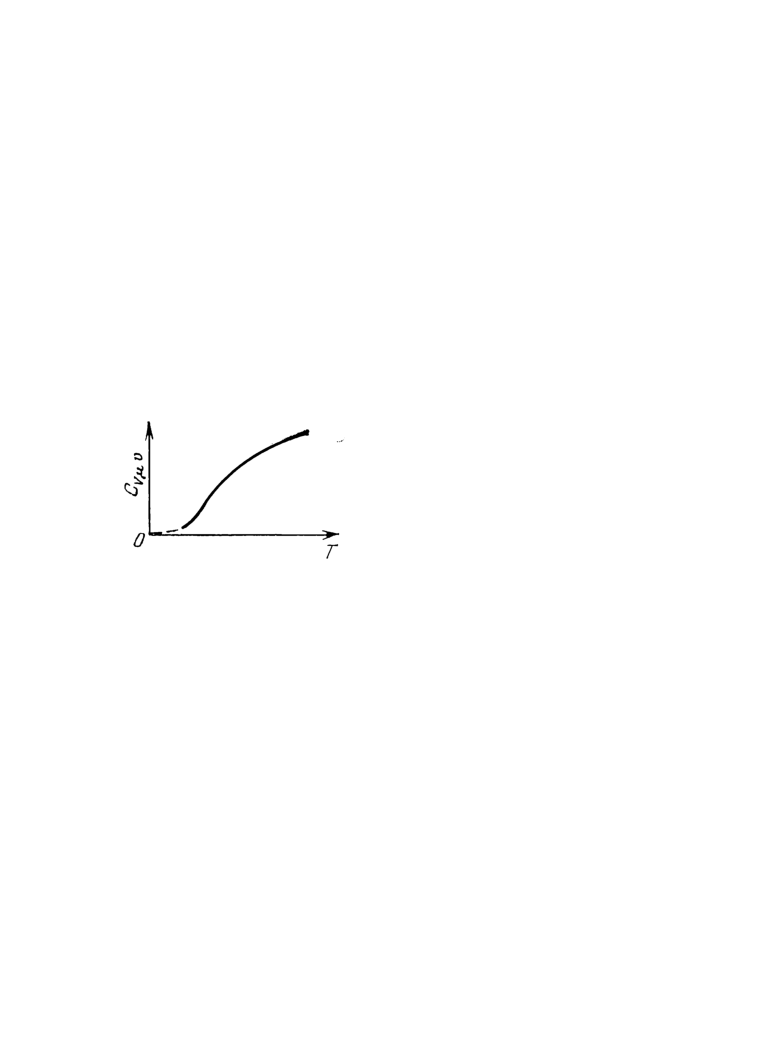
\includegraphics[width=0.8\textwidth]{figs/ch-10/fig-10-07.pdf}
%\input{figs/ch-03/fig-03-01}
%  \vspace{-13pt}
\sidecaption{The dependence $C_{V\mu v} = f(T)$ for diatomic gases.\zhcap{双原子气体的 $C_{V\mu v} = f(T)$ 关系。}\label{fig-10-07}}
\end{marginfigure}

\subsection{}\label{10.7.5} As a first approximation, the rotary motion of diatomic molecules can be dealt with as the motion of a rigid dumbbell which rotates about its centre of mass with the moment of inertia $I = m_{1}m_{2}r_{0}^{2}/(m_{1} + m_{2})$, where $m = m_{1}m_{2}/(m_{1}+ m_{2})$ is the reduced mass of the molecule ($m_{1}$ and $m_{2}$ are the masses of the two atoms), and $r_{0}$ is the distance between the atoms in the molecule. The energy of such a system is
\zhpar{作为第一近似，双原子分子的转动可视为刚性哑铃绕其质心的转动，其转动惯量为 $I = m_{1}m_{2}r_{0}^{2}/(m_{1} + m_{2})$，其中 $m = m_{1}m_{2}/(m_{1}+ m_{2})$ 为分子的约化质量（$m_{1}$ 和 $m_{2}$ 为两原子的质量），$r_{0}$ 为分子中两原子之间的距离。该系统的能量为}
\begin{equation*}%
E^{\text{m}}_{\text{r}} = \frac{h^{2}}{8 \pi I} J (J+1),
\end{equation*}
where $J$ is a quantum number that assumes the values $J = 0, \,1,\, 2, \ldots$ difference $\Delta E^{\text{m}}_{\text{r}}$ between the energies of two adjacent rotational energy levels is
\zhpar{式中 $J$ 为量子数，取值为 $J = 0, \,1,\, 2, \ldots$。相邻两个转动能级的能量差 $\Delta E^{\text{m}}_{\text{r}}$ 为}
\begin{equation*}%
\Delta E^{\text{m}}_{\text{r}} = \frac{2h^{2}}{8 \pi^{2} I} (J+1),
\end{equation*}
The value of $\Delta E^{\text{m}}_{\text{r}}$ is less than $E^{\text{m}}_{\text{v}}$ by a factor of 800 to 1000.
\zhpar{$\Delta E^{\text{m}}_{\text{r}}$ 的数值比 $E^{\text{m}}_{\text{v}}$ 小 800 至 1000 倍。}

At ordinary temperatures $\Delta E^{\text{m}}_{\text{r}} \ll kT$ for diatomic and certain polyatomic gases (water vapour, methane, etc.), and the quantization of the energy of rotary motion of the molecules can be ignored. Under these conditions, the principle of equipartition of energy \ssect{10.6.4} can be applied in calculating the contri­bution of rotary motion to the heat capacity.
\zhpar{在通常温度下，对于双原子气体及某些多原子气体（如水蒸气、甲烷等），$\Delta E^{\text{m}}_{\text{r}} \ll kT$，此时可以忽略分子转动能量的量子化。在这种条件下，计算转动运动对热容的贡献时可以应用能量均分原理 \ssect{10.6.4}。}

The contribution of rotary motion of diatomic molecules to the internal energy and heat capacity per mole equals:
\zhpar{双原子分子的转动运动对每摩尔的内能和热容的贡献为：}
\begin{enumerate}[label=(\alph*)]
\item At high temperatures $(T \gg h^{2}/8\pi^{2}kI)$
\zhpar{在高温（$T \gg h^{2}/8\pi^{2}kI$）时：}

\begin{align*}%
U_{r} & \approx N_{A} kT \left(1 -  \frac{h^{2}}{24\pi^{2}I kT} \right), \qand \\ 
C_{V \mu r} & \approx N_{A}k = R.
\end{align*}
The heat capacity $C_{V \mu r}$ at high temperatures has a value following from the principle of equipartition of energy \ssect{10.6.4}. 
\zhpar{高温下热容 $C_{V \mu r}$ 的值与由能量均分原理得出的结果一致 \ssect{10.6.4}。}
\item At low temperatures $(T \ll h^{2}/8\pi^{2}kI)$
\zhpar{在低温（$T \ll h^{2}/8\pi^{2}kI$）时：}
\begin{align*}%
U_{r} & \approx \frac{3 h^{2} N_{A}}{4 \pi^{2} I} \exp \left(- \frac{h^{2}}{4\pi^{2}I kT} \right),  \\
C_{V \mu r} & \approx 3 \left( \frac{h^{2}}{4 \pi^{2}I} \right) \frac{N_{A}}{kT^{2}} \exp \left(- \frac{h^{2}}{4\pi^{2}I kT} \right).
\end{align*}
as $T \to 0$, the heat capacity $ C_{V \mu r} \to 0$ \ssect{10.7.4}. The general shape of the curve representing the dependence $C_{V \mu r} = f (T)$ is the same as that in \figr{fig-10-07}.
\zhpar{当 $T \to 0$ 时，热容 $C_{V \mu r} \to 0$ \ssect{10.7.4}。$C_{V \mu r} = f (T)$ 曲线的总体形状与 \figr{fig-10-07} 所示曲线相同。}
\end{enumerate}

As the gas cools, the reduction in the energy of its molecules leads to a reduction in the number of molecules transferring to higher rotational energy levels. At sufficiently low tem­peratures, the rotation of the molecules in a gas practically cannot be excited, and rotational degrees of freedom make no contribution to the heat capacity of the gas. The heat capa­cities of all gases at low temperatures become the same as for monatomic gases whose molecules have no rotational degrees of freedom.
\zhpar{气体冷却时，分子能量的降低会使跃迁到较高转动能级的分子数减少。在足够低的温度下，气体分子的转动几乎不能被激发，转动自由度对气体热容没有贡献。此时，各种气体在低温下的热容都与不具有转动自由度的单原子气体相同。}

\subsection{}\label{10.7.6} At extremely high temperatures, of the order of tens of thousands of degrees, the heat capacity is increased. This is associated with the fact that the value of $kT$ under such conditions becomes comparable, in order of magnitude, with $\Delta E_{\text{e}}^{\text{m}}$, the change in the energy of the electrons in their transition from lower to higher energy levels. Moreover, at high tem­peratures the processes of dissociation and ionization of the gases make contributions to their heat capacities.
\zhpar{在数万度量级的极高温度下，热容会增大。这是因为在这样的条件下，$kT$ 的数量级与电子从较低能级跃迁到较高能级时的能量变化 $\Delta E_{\text{e}}^{\text{m}}$ 相当。此外，在高温下，气体的离解和电离过程也会对其热容产生贡献。}

\section{Transport Phenomena in Gases}
\label{sec-10.8}
\zhtitle{气体中的输运现象}

\subsection{}\label{10.8.1} \redem{Transport phenomena} unite a group of processes pertain­ ing to non-uniformities in the density, temperature or velocity of ordered motion of various layers of a substance. The equalization of these non-uniformities leads to transport phenomena. Transport phenomena include diffusion, internal friction and heat conduction.
\zhpar{\redem{输运现象}包括一组与物质中密度、温度或各层有序运动速度的不均匀性有关的过程。这些不均匀性趋于均匀会引起输运现象。输运现象包括扩散、内摩擦和热传导。}

\subsection{}\label{10.8.2} Transport phenomena in gases and liquids consist of ordered directional mass transport in these substances (diffusion), momentum transport (internal friction) and internal energy transport (heat conduction). In gases these phenomena violate the completely random motion of the molecules and Maxwell's molecular velocity distribution \ssect{10.3.2}. Deviations from the Maxwell law can be explained by the directional transport of the physical characteristics of the substance in such phenomena. In the simplest cases of one-dimensional transport phenomena, the physical quantities that govern them depend on only a single Cartesian coordinate.
\zhpar{气体和液体中的输运现象表现为这些物质中的定向质量输运（扩散）、动量输运（内摩擦）和内能输运（热传导）。在气体中，这些现象破坏了分子的完全无规则运动以及麦克斯韦分子速度分布 \ssect{10.3.2}。麦克斯韦定律的这种偏离，可以用这些现象中物质物理特性的定向输运来解释。在一维输运现象的最简单情形中，决定输运过程的物理量仅依赖于单一的笛卡儿坐标。}

\subsection{}\label{10.8.3} \redem{Diffusion} is the spontaneous interpenetration and mixing of the particles of two adjoining gases, liquids or solids. In chemically pure gases at constant temperature, diffusion occurs owing to differing densities in various parts throughout the volume bf the gas. In a mixture of gases, diffusion is caused by the difference in the densities of the various gases at various parts of the volume of the gas mixture.
\zhpar{\redem{扩散}是相邻的两种气体、液体或固体的粒子自发地相互渗透和混合。在化学纯净的气体中，温度恒定时，扩散是由于气体各部分密度不同而发生的。在气体混合物中，扩散是由于混合气体各部分中各种气体的密度差异引起的。}

In a chemically homogeneous gas the phenomenon of diffusion consists in the transport of a mass of the gas from places with higher density to places with lower density. This phenomenon obeys \redem{Fick's law}:
\zhpar{在化学均匀的气体中，扩散现象表现为气体质量从高密度处向低密度处的输运。该现象服从\redem{菲克定律}：}
\begin{equation*}%
m_{\text{sec}} = - D \, \dv{\rho}{x}.
\end{equation*}
Here $m_{\text{sec}}$ is the \redem{specific mass flow} and is numerically equal to the mass that passes by diffusion in unit time through a plane surface of unit area located perpendicular to the direction the substance is being transported, $\rho$ is the density of the gas, and $D$ is the \redem{diffusion coefficient}. The derivative $\dd p / \dd x$ is numer­ically equal to the density gradient, i.e. the change in density per unit length. The diffusion coefficient is numerically equal to the specific mass flow at unit density gradient. The minus sign in Fick's law indicates that mass transport takes place in the direction of decreasing density.
Another form of Fick's law is
\zhpar{式中 $m_{\text{sec}}$ 为\redem{比质量流}，在数值上等于单位时间内通过垂直于物质输运方向的单位面积平面所输运的扩散质量；$\rho$ 为气体密度，$D$ 为\redem{扩散系数}。导数 $\dd p / \dd x$ 在数值上等于密度梯度，即单位长度上的密度变化。扩散系数在数值上等于单位密度梯度下的比质量流。菲克定律中的负号表明，质量输运沿密度减小的方向进行。菲克定律的另一种形式为}
\begin{equation*}%
j  = - D \, \dv{n_{0}}{x},
\end{equation*}
where $j = m_{\text{sec}}/m$ is the density of the molecular flow in diffusion, i.e. the number of molecules diffusing in unit time through the surface indicated in the first form of Fick's law, $n_{0}$ is the molecular concentration, equal to the number of molecules per unit volume, and $m$ is the mass of one molecule, so that $\rho = n_{0} m$.
\zhpar{式中 $j = m_{\text{sec}}/m$ 为扩散中分子流的密度，即单位时间内通过上述第一种形式菲克定律所指表面的扩散分子数；$n_{0}$ 为分子浓度，即单位体积内的分子数；$m$ 为单个分子的质量，因而 $\rho = n_{0} m$。}

The expression obtained in the kinetic theory of gases for the diffusion coefficient is
\zhpar{气体动理论得到的扩散系数表达式为}
\begin{equation*}%
D = \frac{1}{3} \expval{u}\, \expval{\lambda},
\end{equation*}
where $\expval{u}$ is the arithmetic mean velocity of thermal motion of the molecules \ssect{10.3.6}, and $\expval{\lambda}$ is the mean free path \ssect{10.5.1}. 
\zhpar{式中 $\expval{u}$ 为分子热运动的算术平均速率 \ssect{10.3.6}，$\expval{\lambda}$ 为平均自由程 \ssect{10.5.1}。}

\subsection{}\label{10.8.4} \redem{Internal friction} (\redem{viscosity}) is the occurrence of friction forces between layers of a gas or liquid that flow parallel to one another at different speeds. A layer flowing faster exerts an accelerating force on a slower layer. On the other hand, a slow layer retards a faster flowing layer of fluid. The forces of internal friction (viscosity) are directed tangent to the contacting surfaces of the layers. The cause of viscosity (as internal friction in gases and liquids is more commonly called) is the superposition of ordered motion of layers of fluid at various velocities $\vb{v}$ and the thermal random motion of the molecules at velocities depending upon the temperature. 
\zhpar{\redem{内摩擦}（\redem{黏性}）是指彼此以不同速度平行流动的气体或液体层之间产生摩擦力的现象。较快流动的层对较慢的层施加加速作用力；另一方面，较慢的层阻滞较快流动的流体层。内摩擦力（黏性力）与接触层的表面相切。气体和液体中的内摩擦通常称为黏性，其成因是各层流体以不同速度 $\vb{v}$ 的有序运动与分子无规热运动的叠加，而分子无规热运动的速度取决于温度。}

The random motion of the molecules transfers them from layer $B$ flowing at the velocity $\vb{v}_{2}$ into layer $A$ flowing at the velocity $\vb{v}_{1} $(\figr{fig-10-08}). This leads to transport of momenta $m\vb{v}$ of ordered motion of the molecules. When $\vb{v}_{1}> \vb{v}_{2}$, the molecules that entered layer $A$ from layer $B$ have their velocities of ordered motion accelerated by collisions with the molecules from the new layer. This slows down the velocities of ordered motion of the molecules in layer $A$. On the other hand, molecules passing from faster layer $A$ to slower layer $B$ have higher mo­menta $m\vb{v}_{1}$ so that the inter-molecular collisions in layer $B$ accelerate the motion of its molecules.
\zhpar{分子的无规运动使分子从以速度 $\vb{v}_{2}$ 运动的 $B$ 层迁移到以速度 $\vb{v}_{1}$ 运动的 $A$ 层（\figr{fig-10-08}）。这导致了分子有序运动动量 $m\vb{v}$ 的输运。当 $\vb{v}_{1}> \vb{v}_{2}$ 时，从 $B$ 层进入 $A$ 层的分子，在与新层中分子碰撞时，其有序运动速度会增大，这减慢了 $A$ 层中分子有序运动的速度。另一方面，从较快的 $A$ 层进入较慢的 $B$ 层的分子具有较大的动量 $m\vb{v}_{1}$，因此分子间的碰撞会加快 $B$ 层分子的运动。}

\begin{marginfigure}[-3cm]%[!ht]
%\begin{wrapfigure}{r}{0.5\linewidth}
\centering
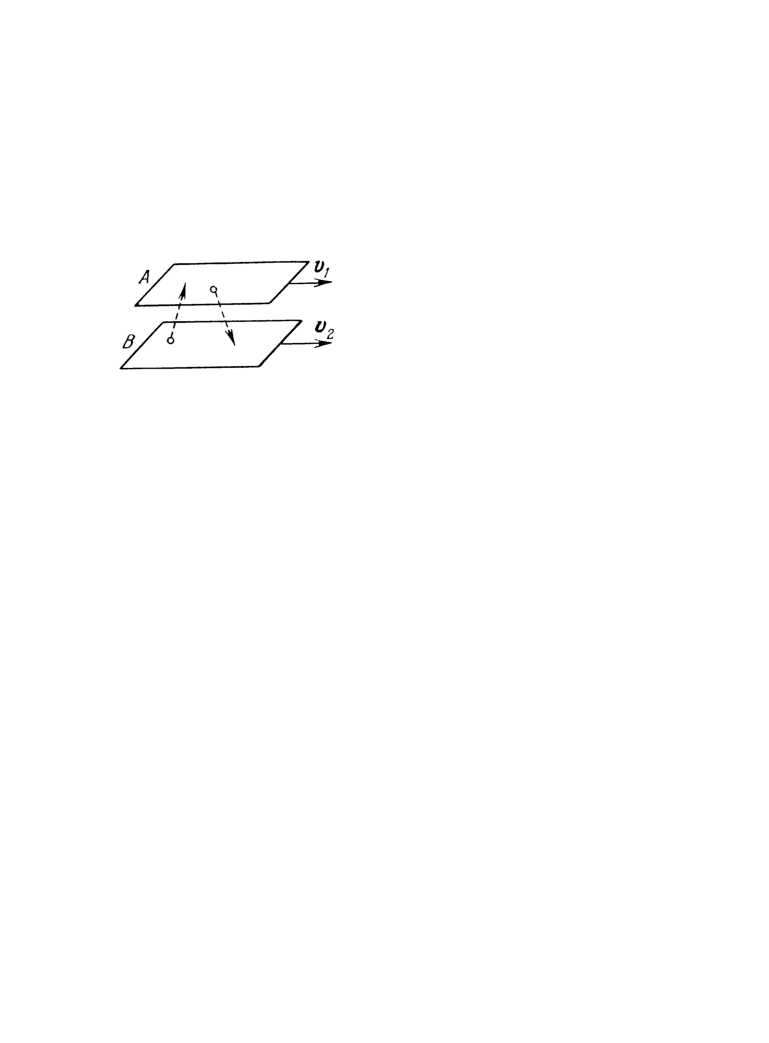
\includegraphics[width=0.8\textwidth]{figs/ch-10/fig-10-08.pdf}
%\input{figs/ch-03/fig-03-01}
%  \vspace{-13pt}
\sidecaption{The random motion of the molecules transfers them between layer of a fluid.\zhcap{分子的无规运动使分子在流体各层之间迁移。}\label{fig-10-08}}
\end{marginfigure}
The phenomenon of viscosity is described by the \redem{Newtonian friction law}:
\zhpar{黏性现象由\redem{牛顿内摩擦定律}描述：}
\begin{equation*}%
\tau = - \eta \dv{v}{n},
\end{equation*}
where $\tau$ is the \redem{friction stress}, i.e. the physical quantity equal nu­merically to the force of internal friction acting per unit area of the surface of the layer, $\dd v/\dd n$ is the velocity gradient, i.e. the variation in the velocity of layer motion per unit length in the direction of the inner normal $\vb{n}$ to the layer surface. The internal frictional force is opposite in direction to the derivative of the gas velocity vector $\vb{v}$ with respect to $\vb{n}$. The quantity $\eta$ is called the \redem{coefficient of dynamic viscosity} (or just the \redem{viscosity}). It is numerically equal to the friction stress at a velocity gradient equal to unity.
\zhpar{式中 $\tau$ 为\redem{摩擦应力}，即在数值上等于作用于层表面单位面积上的内摩擦力的物理量；$\dd v/\dd n$ 为速度梯度，即沿层表面内法线 $\vb{n}$ 方向单位长度上层运动速度的变化。内摩擦力的方向与气体速度矢量 $\vb{v}$ 对 $\vb{n}$ 的导数方向相反。量 $\eta$ 称为\redem{动力黏性系数}（或简称\redem{黏性}），它在数值上等于速度梯度为单位值时的摩擦应力。}

The \redem{coefficient of kinematic viscosity} is the quantity $\nu = \eta/\rho$, where $\rho$ is the density of the substance. The coefficient of dynamic viscosity is calculated by the equa­tion
\zhpar{\redem{运动黏性系数}为量 $\nu = \eta/\rho$，其中 $\rho$ 为物质的密度。动力黏性系数由下列公式计算：}
\begin{equation*}%
\eta = \frac{1}{3} \expval{u}\, \expval{\lambda} \, \rho,
\end{equation*}
where $\expval{u}$ is the arithmetic mean velocity of thermal motion of the molecules \ssect{10.3.6}, and $\expval{\lambda}$ is their mean free path \ssect{10.5.1}. The coefficient of dynamic viscosity is independent of the pressure (or density) of the gas since $\expval{\lambda} \propto 1/\rho$. This can be explained by the fact that in an isothermal increase in the density of a gas, for example, by two times, the number of carriers of momenta is doubled, but each molecule (or atom) travels only one half the distance without a collision and carries only one half as much momentum. Hence, all in all, momenta transport remains unchanged.
\zhpar{式中 $\expval{u}$ 为分子热运动的算术平均速率 \ssect{10.3.6}，$\expval{\lambda}$ 为其平均自由程 \ssect{10.5.1}。由于 $\expval{\lambda} \propto 1/\rho$，动力黏性系数与气体的压强（或密度）无关。这可以这样解释：在温度不变时将气体密度增大为两倍，动量载体的数目也增为两倍，但每个分子无碰撞飞越的距离只有原来的一半，携带的动量也只有原来的一半。因此，总的动量输运保持不变。}

\subsection{}\label{10.8.5} The third transport phenomenon, \redem{heat conduction}, occurs under the condition that a difference in temperature exists in a body in a certain direction. For instance, the two opposing walls of a vessel holding a gas can have different temperatures that are maintained by external sources. Then the gas molecules at various locations throughout the volume have different average kinetic energies \ssect{10.2.4}. Under such conditions, the random thermal motion of the molecules leads to directional energy transport (or transfer) in the form of heat \ssect{9.2.6}. Molecules passing from the heated parts of the volume of gas to the colder parts yield some of their average kinetic energy to the surrounding molecules in the process of molecular collisions. Slow molecules, on the contrary, increase their average kinetic energy, in passing from the less heated to the more heated parts of the gas, owing to collisions with molecules having higher velocities.
\zhpar{第三种输运现象\redem{热传导}发生在物体中沿某一方向存在温差的条件下。例如，容纳气体的容器两个相对的器壁可以保持不同的温度，并由外部热源维持。此时，气体不同位置的分子具有不同的平均动能 \ssect{10.2.4}。在这种条件下，分子的无规热运动导致能量以热量形式定向输运（或传递） \ssect{9.2.6}。从气体较热部分运动到较冷部分的分子，在碰撞过程中将其部分平均动能传递给周围的分子。相反，较慢的分子从较冷部分进入较热部分时，通过与速度较大的分子碰撞而增加其平均动能。}

In one-dimensional heat conduction, when the temperature of the gas depends only on a single coordinate $T = T (x)$, energy transfer in the form of heat proceeds along the $OX$ axis according to the \redem{Fourier law} of heat conduction (Fourier heat equation): 
\zhpar{当气体温度仅依赖于单一坐标 $T = T (x)$ 时（一维热传导），能量以热量形式沿 $OX$ 轴按\redem{傅里叶热传导定律}（即傅里叶热传导方程）传递：}
\begin{equation*}%
q_{\textrm{sec}} = - K \dv{T}{x},
\end{equation*}
where $q_{\textrm{sec}}$ is the \redem{specific rate of heat flow}, a physical quantity numerically equal to the energy transmitted in the form of heat in unit time through a plane surface of unit area located perpendicular to the direction of energy transport. The quantity $K$ is called the \redem{thermal conductivity}. It is numerically equal to the specific rate of heat flow at the temperature gradient $\dd T / \dd x$ (the change in temperature over unit length) equal to unity. The minus sign in the Fourier law indicates that in heat conduction energy is transported in the direction of decreasing temperatures.
\zhpar{式中 $q_{\textrm{sec}}$ 为\redem{比热流}，是一个物理量，在数值上等于单位时间内通过垂直于能量传输方向的单位面积平面所传递的热量。量 $K$ 称为\redem{热导率}，在数值上等于温度梯度 $\dd T / \dd x$（单位长度上的温度变化）为单位值时的比热流。傅里叶定律中的负号表明，热传导中能量沿温度降低的方向输运。}


According to the kinetic theory of gases, the thermal conduc­tivity is equal to
\zhpar{根据气体动理论，热导率等于}
\begin{equation*}%
K = \frac{1}{3} \expval{u}\, \expval{\lambda} \, c_{V} \rho,
\end{equation*}
where $c_{V}$ is the specific heat at constant volume \ssect{9.5.4}. The other quantities are defined in \ssect{10.8.4}. It follows from the last equation that the thermal conductivity is inde­pendent of the gas density. The reasons are similar to those given in \ssect{10.8.4} to explain why $\eta$ is independent of the density.
\zhpar{式中 $c_{V}$ 为定容比热容 \ssect{9.5.4}，其余量的定义见 \ssect{10.8.4}。由上式可知，热导率与气体密度无关。其理由与 \ssect{10.8.4} 中解释 $\eta$ 与密度无关时所给出的理由相似。}

\subsection{}\label{10.8.6} The laws of transport phenomena, given in the subsec­tions \ssect{10.8.3}, \ssect{10.8.4} and \ssect{10.8.5}, can be written in another form:
\zhpar{\ssect{10.8.3}、\ssect{10.8.4} 和 \ssect{10.8.5} 中给出的输运现象规律，也可以写成另一种形式：}
\begin{align*}%
\dd M & = - D \,\dv{\rho}{x}\, \dd S \,\dd t,\\
\dd F & = - \eta \,\dv{v}{x}\, \dd S \,\dd t,\\
\dd Q & = - K \,\dv{T}{x} \dd S \dd t.
\end{align*}
Here $\dd M$ is the mass transported in diffusion during the time $\dd t$ through the element of area $\dd S$, located perpendicular to the direction of diffusion; $\dd Q$ is the amount of energy transported in the form of heat during the time $\dd t$ through the same element of area $\dd S$, located perpendicular to the $OX$ axis; and $\dd F$ is the force of internal friction (viscous force) exerted on an ele­ment of surface of the layer having the area $\dd S$. The other quantities are defined in the subsections mentioned above.
\zhpar{式中 $\dd M$ 为在时间 $\dd t$ 内通过垂直于扩散方向的面积元 $\dd S$ 所输运的扩散质量；$\dd Q$ 为在时间 $\dd t$ 内以热量形式通过垂直于 $OX$ 轴的同一面积元 $\dd S$ 所输运的能量；$\dd F$ 为作用在面积为 $\dd S$ 的层表面单元上的内摩擦力（黏性力）。其余量的定义见上述各小节。}

\begin{table}
\begin{footnotesize}
\begin{tabular}{p{2cm}p{2cm}p{3cm}p{2.75cm}}
\toprule
Phenomenon & Transported physical quantity & Transport equa­tion & Formula for the transport coefficient \\
\midrule
Diffusion & Mass & $\dd M = - D \,\dv{\rho}{x}\, \dd S \,\dd t$ & $D = \frac{1}{3} \expval{u}\, \expval{\lambda}$ \\[5pt]
Internal friction (viscosity) & Momentum &$\dd F = - \eta \,\dv{v}{x}\, \dd S \,\dd t$ & $\eta = \frac{1}{3} \expval{u}\, \expval{\lambda} \, \rho$\\
Heat con­duction & Energy in the form of heat & $\dd Q  = - K \,\dv{T}{x} \dd S \,\dd t$ & $K = \frac{1}{3} \expval{u}\, \expval{\lambda} \, c_{V} \rho$\\
\bottomrule
\end{tabular}
\end{footnotesize}
\sidecaption{Information on transport phenomena.\zhcap{输运现象的有关信息。}
\label{tbl-10-01}}
\end{table}
\subsection{}\label{10.8.7} Simple relations exist between the transport coefficients:
\zhpar{输运系数之间存在下列简单的关系：}
\begin{equation*}%
\eta = \rho \, D, \quad \frac{K}{\eta c_{V}} = 1.
\end{equation*}
If any one of the transport coefficients is known the others can be found by these formulas (for known values of $\rho$ and $c_{V}$). When the coefficients are known, such vital characteristics of a gas can be determined as the mean free path \ssect{10.5.1} of its molecules and the effective diameter of the molecules \ssect{8.4.1}. Information on transport phenomena is listed in Table \ref{tbl-10-01}.
\zhpar{若已知任一输运系数，则其他系数可由这些公式求得（已知 $\rho$ 和 $c_{V}$ 时）。当输运系数已知时，可以确定气体的一些重要特征量，如分子的平均自由程 \ssect{10.5.1} 和分子的有效直径 \ssect{8.4.1}。输运现象的有关信息列于表 \ref{tbl-10-01} 中。}

\section{Properties of Rarified Gases}
\label{10.9}
\zhtitle{稀薄气体的性质}

\subsection{}\label{10.9.1} A gas in said to be \redem{rarified} (a \redem{dilute gas}) if its density is so low that the mean free path $\expval{\lambda}$ of the molecules is com­ parable to the linear dimensions d of the vessel confining the gas. Such a state of a gas is also called a \redem{vacuum}. The degrees of vacuum of gases are classified as ultrahigh $(\expval{\lambda} \gg d)$, high $(\expval{\lambda} > d)$, medium $(\expval{\lambda} \leqslant d)$ and low $(\expval{\lambda} \gg d)$. The proper­ties of rarified gases differ from those of non-rarified gases only for the first three of these degrees of vacuum. This is evident from Table \ref{tbl-10-02} which lists certain characteristics for the various degrees.
\zhpar{当气体的密度很低，以致其分子的平均自由程 $\expval{\lambda}$ 与容纳气体的容器线性尺寸 $d$ 相当时，该气体称为\redem{稀薄气体}（亦称\redem{低密度气体}）。这种状态的气体也称为\redem{真空}。气体的真空度分为超高真空 $(\expval{\lambda} \gg d)$、高真空 $(\expval{\lambda} > d)$、中真空 $(\expval{\lambda} \leqslant d)$ 和低真空 $(\expval{\lambda} \gg d)$。只有前三种真空度下，稀薄气体的性质才与非稀薄气体的性质不同。表 \ref{tbl-10-02} 列出了各真空度的某些特征，由此可以看出这一点。}


% \usepackage{multirow}


\begin{table*}
\centering
\begin{footnotesize}
\begin{tabular}{p{2cm}p{1.75cm}p{1.75cm}p{1.75cm}p{1.75cm}}
\toprule
\multirow{2}{*}{Characteristic}   & \multicolumn{4}{c}{Vacuum}   \\
%\midrule
 & Low & Medium & High & Ultrahigh  \\
\midrule
Pressure &   \num{760} to \num{1}  &    \num{1} to \num{d-3}    &    \num{d-3} to  \num{d-7}  &   \num{d-8} and less\\[5pt]
Number of molecules in unit volume (per \si{\meter\cubed}) &    \num{d25} to  \num{d22}  &   \num{d22} to  \num{d19}     &    \num{d19} to  \num{d13}  & \num{d13} and less            \\[5pt]
Dependence
of coeffic­ients $K$ and $\eta$ on the pres­sure          &   None  &     Pressure dependence is deter­mined by the parameter $\expval{\lambda}/d$  & Directly proportional to pressure      &  Heat conduction and viscosity are practically absent         \\
\bottomrule                          
\end{tabular}
\end{footnotesize}
\sidecaption[][2cm]{Properties of gas in different vacuums.\zhcap{不同真空度下气体的性质。}
\label{tbl-10-02}}
\end{table*}


\subsection{}\label{10.9.2} \redem{In the stale of a high vacuum} (\ssect{10.9.1}) a reduction in the density of a rarified gas leads to a corresponding decrease in the number of particles without changing $\lambda$). This, conse­quently, reduces the number of carriers of momentum or inter­nal energy in viscosity and heat conduction. The transport coefficients in these phenomena are directly proportional to the gas density (cf. \ssect{10.8.4} and \ssect{10.8.5}). Internal friction is essentially absent in highly rarified gases. Instead, only exter­nal friction exists between the moving gas and the walls of the vessel. This is due to the fact that the molecules change their momentum only in interacting with the walls. Under these conditions, as a first approximation, the friction stress is proportional to the density of the gas and velocity of its motion (cf. Sect. \ssect{10.8.4}). The specific rate of heat flow in highly rarified gases is proportional to the temperature difference and to the gas density (cf. Sect. \ssect{10.8.5}).
\zhpar{\redem{在高真空状态下}（\ssect{10.9.1}），稀薄气体密度的降低导致粒子数相应减少（而 $\lambda$ 保持不变）。因此，黏性和热传导中动量或内能的载体数目也随之减少。这些现象中的输运系数与气体密度成正比（参见 \ssect{10.8.4} 和 \ssect{10.8.5}）。在高度稀薄的气体中，内摩擦基本不存在，取而代之的是运动气体与容器器壁之间只存在外摩擦。这是因为分子只有在与器壁相互作用时才改变其动量。在这些条件下，作为一级近似，摩擦应力与气体密度及其运动速度成正比（参见 Sect. \ssect{10.8.4}）。高度稀薄气体中的比热流与温差及气体密度成正比（参见 Sect. \ssect{10.8.5}）。}


\subsection{}\label{10.9.3} A steady state of a rarified gas, contained in two vessels connected by a narrow tube, is possible under the condition of equality of the counterflow of particles passing between the vessels: $n_{1}\expval{u_{1}} = n_{2} \expval{u_{2}}$, where $n_{1}$ and $n_{2}$ are the numbers of molecules per \si{\centi\meter\cubed} in the two vessels, and $\expval{u_{1}}$ and $\expval{u_{2}}$ are their arithmetic mean velocities \ssect{10.3.6}.
\zhpar{稀薄气体若装在两个由细管相连的容器中，只有当两容器之间粒子的反向流动数量相等，即 $n_{1}\expval{u_{1}} = n_{2} \expval{u_{2}}$ 时，系统才能达到稳定状态。其中 $n_{1}$ 和 $n_{2}$ 分别为两容器中每立方厘米内的分子数，$\expval{u_{1}}$ 和 $\expval{u_{2}}$ 为两容器中分子的算术平均速率 \ssect{10.3.6}。}

If $T_{1}$ and $T_{2}$ are the gas temperatures in the two vessels, the preceding condition for a steady state can be rewritten in the form of an equation that expresses the \redem{Knudsen effect}:
\zhpar{若 $T_{1}$ 和 $T_{2}$ 为两容器中的气体温度，则上述稳定态条件可以改写为表示\redem{克努森效应}的方程：}
\begin{equation*}%
\frac{p_{1}}{p_{2}} = \sqrt{\frac{T_{1}}{T_{2}}}.
\end{equation*}

where $p_{1}$ and $p_{2}$ are the pressures of the rarified gas in the two vessels.
\zhpar{式中 $p_{1}$ 和 $p_{2}$ 分别为两容器中稀薄气体的压强。}
